\documentclass[10pt,a5paper]{book}

\usepackage{polski}
\usepackage[T1]{fontenc}
\usepackage[utf8]{luainputenc}
\usepackage[twoside, a5paper,top=1.5cm, bottom=1.5cm, left = 1.0cm, right=1.0cm, bindingoffset=0.5cm]{geometry}
%\usepackage{amsmath}
\usepackage{bm}
\usepackage{graphicx}
%\usepackage{indentfirst}
\usepackage[font={small}]{caption}
\usepackage{multicol}
\usepackage{xfrac}
\usepackage[space]{grffile}
\usepackage{tgtermes}
\usepackage{titlesec, blindtext, color, colortbl}
\usepackage{tikz}
\usepackage[compat=1.1.0]{tikz-feynman}
\usepackage[bottom]{footmisc}
\usepackage{subcaption}
\usepackage[hidelinks]{hyperref}
\usepackage{makecell}
\usepackage{array}
\usepackage{xcolor}
\usepackage{marvosym}
\usepackage{cite}
\usepackage{fontspec-luatex}
\usepackage{libertinus-otf}
\usepackage[normalem]{ulem}
\usepackage{gensymb}
\usepackage{multirow}
\usepackage{booktabs}
\usepackage{listings}
\usepackage{afterpage}
\usepackage{paracol}
\usepackage{slashed}
\usepackage{pifont}
\usepackage{fontspec}
\usepackage[mathscr]{euscript}
\usepackage{fancyhdr}
\usepackage{enumitem}
\usepackage{pgfornament}

\renewcommand{\footrulewidth}{1pt}

\pagestyle{fancy}
\fancyhf{}
\fancyhead[LE,RO]{}
\fancyhead[CE,CO]{}
\fancyfoot[LE,RO]{\thepage}
\fancyfoot[RE,LO]{{\small Duszpasterstwo Wiernych Tradycji Łacińskiej w Archidiecezji Wrocławskiej}}

\graphicspath{{Figures/}}

\setlength\parindent{0pt}

\titleformat{\section}[hang]{}{}{0pt}{\large\bfseries\centering}
\titleformat{\subsection}[hang]{}{}{0pt}{\large\centering}

\newcommand{\kol}{black}

\newcommand{\textjuni}[1]{{\fontspec{Junicode-Regular}#1}}

\newcommand{\vv}{\textcolor{\kol}{\textjuni{\char"2123. }}}
\newcommand{\rr}{\textcolor{\kol}{\textjuni{\char"211F. }}}
\newcommand{\rrr}{\newline\textcolor{\kol}{\textjuni{~~~~~~\char"211F. }}}
\newcommand{\nn}{\boldmath$\mathscr{N}$.~}

\newcommand{\rubric}[1]{\medskip{\bfseries\color{\kol} #1}\medskip}

\newcommand{\station}[1]{\centering\vspace*{-0.2cm}\small\textit{#1}\bigskip\\}
\newcommand{\proroctwo}[1]{\bigskip{\bfseries\centerline{#1}}\medskip}
\newcommand{\proroctwoo}[2]{\bigskip{\bfseries\centerline{#1}}\smallskip{\color{\kol}\itshape\centerline{#2}}\medskip}

\newcommand{\oremus}[3]{\medskip\centerline{\textbf{#1}}\medskip
	\begin{sloppypar}
		\begin{paracol}{2}
			\setlength{\columnsep}{0em}
			\begin{leftcolumn}
				#2
			\end{leftcolumn}
			\begin{rightcolumn}
				#3
			\end{rightcolumn}
		\end{paracol}
	\end{sloppypar}}

\newcommand{\oremuss}[2]{
	\begin{sloppypar}
		\begin{paracol}{2}
			\setlength{\columnsep}{0em}
			\begin{leftcolumn}
				#1
			\end{leftcolumn}
			\begin{rightcolumn}
				#2
			\end{rightcolumn}
		\end{paracol}
	\end{sloppypar}}


\begin{document}
	
	\thispagestyle{empty}
	
	\begin{center}
		\vspace*{0.5cm}
		
		
		\bfseries\scshape
		\huge WIGILIA \\ ZESŁANIA DUCHA ŚWIĘTEGO \\\medskip
		\Large oraz \\\medskip
		\huge MSZA ŚWIĘTA \\ W DZIEŃ PIĘĆDZIESIĄTNICY \\\bigskip
		\large WEDŁUG KSIĄG LITURGICZNYCH SPRZED 1955 r.
		
		\vfill
		
		\pgfornament[width=7cm]{88}
		
		\vfill	
		
		\begin{figure}[h]
			\centering
			
\includegraphics[width=0.3\linewidth]{logo.jpg}
		\end{figure}
	
		\vfill
		
		{\large Duszpasterstwo Wiernych Tradycji Łacińskiej \\ w Archidiecezji Wrocławskiej}
		
		\bigskip
		
		{\Large \textbf{2019}}
		
		
	\end{center}

%	\afterpage{\null\thispagestyle{empty}\newpage}

	\newpage
	\thispagestyle{empty}
	
	\vspace*{2cm}
	"Oto misterium Pięćdziesiątnicy: Duch Święty oświeca ducha ludzkiego, a objawiając ukrzyżowanego i zmartwychwstałego Chrystusa, wskazuje, na jakiej drodze możemy upodobnić się do Niego, czyli być «wyrazem i narzędziem miłości, która od Niego emanuje» (Deus caritas est, 33). Razem z Maryją, tak jak w chwili swych narodzin, Kościół modli się dzisiaj: «Przyjdź, Duchu Święty! Przyjdź, Duchu Święty, napełnij serca swoich wiernych i zapal w nich ogień swojej miłości!» Amen."
	
	\bigskip
	
	\hfill \textit{Benedykt XVI, Homilia  w uroczystość Zesłania Ducha Świętego 2006}
	
	\vspace*{\fill}
	
	\hrulefill
	
	{\footnotesize 
	Niniejszy mszalik przygotowany jest w celu wyjaśnienia obrzędów i edukacji liturgicznej wiernych. Teksty liturgiczne wraz z tłumaczeniami oraz grafiki pochodzą z:
	
	\begin{itemize}[leftmargin=*]
		\item \textit{Mszału Rzymskiego z dodaniem nabożeństw nieszpornych} autorstwa O. Gaspara Lefebvre (Poznań 1932)
		\item \textit{Mszału Rzymskiego} autorstwa benedyktynów tynieckich (Poznań 1963)
		\item \textit{Missale Romanum} wyd. Typis Polyglotis Vaticanis (1927) oraz Pustet (1899)
	\end{itemize}

	W niektórych przypadkach wykorzystano cyfrową wersję powyższych tekstów opublikowaną na portalu \url{divinumofficium.com}.
	
	\medskip
	
	Krótki cytat z homilli Benedykta XVI pochodzi z \textit{L'Osservatore Romano} (8/2006)
	
	\medskip
	
	Teksty czytań opatrzone komentarzem i wyjaśnieniem zaczerpnięto z \textit{Biblii Tysiąclecia Online} (Poznań 2003). Zostały one wykorzystane na mocy prawa cytatu. (art. 29. Ustawy o prawie autorskim i prawach pokrewnych) Prawa autorskie do nich posiada wyd. Pallotinum. Tekst Biblii Tysiąclecia jest oficjalnym tekstem Kościoła w Polsce zatwierdzonym do stosowania w liturgii.
	
	\bigskip
	
	opracowanie: M. Rumin, Ł. Wolański, M. Skarupski\\
	nadzór merytoryczny ks. dr Ireneusz Bakalarczyk\\
	skład i łamanie: Michał Siemaszko\\
	
	email: tradycja@archidiecezja.wroc.pl 
	}
	\hrule
	
%	\afterpage{\null\thispagestyle{empty}\newpage}
	\newpage
	
	%%%%%%%%%%%%%%%%%%%%%%%%%%%%%%%%%%%%%%%%%%%%%%%%%%%%%%%%%%%%%%%%%%%%%%%%%%
	
	\fancyhead[CE,CO]{WIGILIA PIĘĆDZIESIĄTNICY}
	
	\begin{figure}[h]
		\centering
		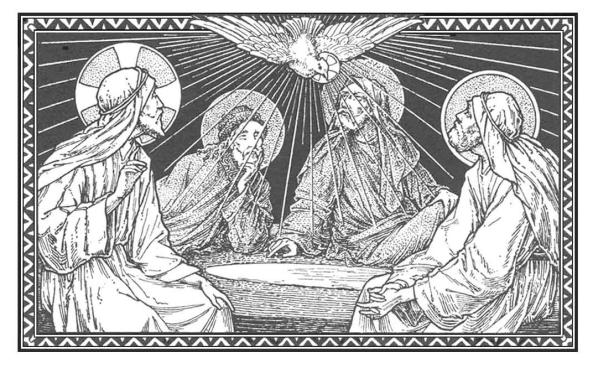
\includegraphics[width=\linewidth]{1.jpg}
	\end{figure}

	\section{SOBOTA W WIGILIĘ ZESŁANIA DUCHA ŚWIĘTEGO}	
		{\station{Stacja u św. Jana na Lateranie}}
		
	
		\rubric{
			„Wtedy wrócili do Jerozolimy z góry, zwanej Oliwną, która leży blisko Jerozolimy, w odległości drogi szabatowej. Przybywszy tam weszli do sali na górze i przebywali w niej: Piotr i Jan, Jakub i Andrzej, Filip i Tomasz, Bartłomiej i Mateusz, Jakub, syn Alfeusza, i Szymon Gorliwy, i Juda, brat Jakuba. Wszyscy oni trwali jednomyślnie na modlitwie razem z niewiastami, Maryją, Matką Jezusa, i braćmi Jego.” (Dz 1, 12-14) 
			
			\medskip
			
			Wigilia Pięćdziesiątnicy to wyjątkowy obchód w tradycyjnym rycie rzymskim. Tego dnia, podobnie jak w czasie Wigilii Paschalnej, dokonuje się poświęcenia źródła chrzcielnego i udziela się sakramentów chrztu i bierzmowania. Tradycja udzielania tych sakramentów w Wigilie Pięćdziesiątnicy pochodzi z pierwszych wieków chrześcijaństwa. Wspominają o tym w swoich pismach papieże św. Syrycjusz (384-399) i św. Leon I (440-461), powołując się na przykład św. Piotra, który w dzień Zesłania Ducha Świętego ochrzcił trzy tysiące osób.}
		
		\newpage
		
		\subsection{LITURGIA SŁOWA --- PROROCTWA}
	
			\rubric{
				Po odmówieniu Nony w chórze, Kapłan i usługujący w szatach koloru fioletowego udają się procesyjnie do ołtarza, oddając mu cześć w zwykły sposób, kapłan całuje ołtarz na środku. Następnie odczytuje się proroctwa bez tytułu, świece na ołtarzu są zgaszone aż do początku Mszy podobnie jak w Wielką Sobotę. Na końcu proroctw odmawia się orację bez \textit{Flectámus génua}. W tym czasie duchowni przyjmują do kościoła katechumenów, pouczają ich, odprawiają ezgorcyzmy i przygotowują ich do przyjęcia Sakramentów Chrztu i Bierzmowania.
				
				Wybrane z kart Starego Testamentu czytania ukazują stopniowy rozwój dzieła Odkupienia i zapowiadają odrodzenie w Chrystusie i zesłanie Ducha Pocieszyciela. Jest to przygotowanie do poświęcenia wody chrzcielnej, w której źródle zaczyna się odrodzenie i nawrócenie człowieka.}
			
				\proroctwoo{Proroctwo I (Rdz 22, 1--19)}{Ofiara Abrahama}
				
				\rubric{
					Pierwsze proroctwo to fragment Księgi Rodzaju. Ukazuje on heroiczną wiarę Abrahama, który wystawiony na bardzo cięż ką próbę okazuje całkowite posłuszeństwo Bogu. Mądrość Abrahama nie jest mądrością ludzką, opartą o wybór tego, co słuszne według rozumu, ale prawdziwą pochodzącą od Boga mądrością, która nakazuje zaufać Stwórcy ze względu na jego Boski Autorytet.}
				
				% Pierwsze czytanie
				W owych dniach Bóg wystawił Abrahama na próbę i rzekł do niego: «Abrahamie!» A gdy on odpowiedział: «Oto
				jestem» powiedział: «Weź twego syna jedynego, którego miłujesz, Izaaka, idź do kraju Moria i tam złóż go w
				ofierze na jednym z pagórków, jakie ci wskażę». Nazajutrz rano Abraham osiodłał swego osła, zabrał z sobą
				dwóch swych ludzi i syna Izaaka, narąbał drzewa do spalenia ofiary i ruszył w drogę do miejscowości, o której mu
				Bóg powiedział. Na trzeci dzień Abraham, spojrzawszy, dostrzegł z daleka ową miejscowość. I wtedy rzekł do
				swych sług: «Zostańcie tu z osłem, ja zaś i chłopiec pójdziemy tam, aby oddać pokłon Bogu, a potem wrócimy do
				was». Abraham, zabrawszy drwa do spalenia ofiary, włożył je na syna swego Izaaka, wziął do ręki ogień i nóż, po
				czym obaj się oddalili.
				Izaak odezwał się do swego ojca Abrahama: «Ojcze mój!» A gdy ten rzekł: «Oto jestem, mój synu» - zapytał: «Oto
				ogień i drwa, a gdzież jest jagnię na całopalenie?» Abraham odpowiedział:
				«Bóg upatrzy sobie jagnię na całopalenie, synu mój». I szli obydwaj dalej. A gdy przyszli na to miejsce, które Bóg
				wskazał, Abraham zbudował tam ołtarz, ułożył na nim drwa i związawszy syna swego Izaaka położył go na tych
				drwach na ołtarzu. Potem Abraham sięgnął ręką po nóż, aby zabić swego syna.
				Ale wtedy Anioł Pański zawołał na niego z nieba i rzekł: «Abrahamie, Abrahamie!» A on rzekł: «Oto jestem».
				Odpowiedział mu: «Nie podnoś ręki na chłopca i nie czyń mu nic złego! Teraz poznałem, że boisz się Boga, bo nie
				odmówiłeś Mi nawet twego jedynego syna».
				Abraham, obejrzawszy się poza siebie, spostrzegł barana uwikłanego rogami w zaroślach. Poszedł więc, wziął
				barana i złożył w ofierze całopalnej zamiast swego syna. I dał Abraham miejscu temu nazwę "Pan widzi". Stąd to
				mówi się dzisiaj: «Na wzgórzu Pan się ukazuje».
				Po czym Anioł Pański przemówił głośno z nieba do Abrahama po raz drugi: «Przysięgam na siebie, wyrocznia
				Pana, że ponieważ uczyniłeś to, a nie oszczędziłeś syna twego jedynego, będę ci błogosławił i dam ci potomstwo
				tak liczne jak gwiazdy na niebie i jak ziarnka piasku na wybrzeżu morza; potomkowie twoi zdobędą warownie
				swych nieprzyjaciół. Wszystkie ludy ziemi będą sobie życzyć szczęścia [takiego, jakie jest udziałem] twego
				potomstwa, dlatego że usłuchałeś mego rozkazu».
				Abraham wrócił do swych sług i wyruszywszy razem z nimi w drogę, poszedł do Beer-Szeby.
				I mieszkał Abraham nadal w Beer--Szebie.
				
				\oremus{Modlitwa}{
					Deus, qui in Abrahæ fámuli tui opere humáno generi
					ob\oe diéntiæ exémpla præbuísti; concéde nobis, et nostræ
					voluntátis pravitátem frángere, et tuórum præceptórum
					rectitúdinem in ómnibus adimplére. Per Dóminum
					nostrum.\\}
					{Boże, któryś w ofierze sługi swego, Abrahama, dał						ludziom przykład posłuszeństwa, spraw abyśmy przełamali złość naszej woli i we wszystkim wypełniali prawe przykazania Twoje.}
					
				\proroctwoo{Proroctwo II (Wj 14, 24--31; 15, 1)}{Przejście Izraela przez Morze Czerwone}

				
				\rubric{
					Drugie proroctwo Wigilii Pięćdziesiątnicy opisuje Przejście Izraelitów przez Morze Czerwone. Było ono
					warunkiem wyzwolenia Izraelitów z niewoli egipskiej i wprowadzenia do Ziemi Obiecanej. Jest to zapowiedź
					chrztu świętego, który wyzwala chrześcijan z jarzma szatana i wprowadza do Świętego Kościoła.}
				
				W owych dniach o świcie spojrzał Pan ze słupa ognia i ze słupa obłoku na wojsko egipskie i zmusił je do ucieczki.
				I zatrzymał koła ich rydwanów, tak że z wielką trudnością mogli się naprzód posuwać. Egipcjanie krzyknęli:
				«Uciekajmy przed Izraelem, bo w jego obronie Pan walczy z Egipcjanami».
				A Pan rzekł do Mojżesza: «Wyciągnij rękę nad morze, aby wody zalały Egipcjan, ich rydwany i jeźdźców».Wyciągnął Mojżesz rękę nad morze, które o brzasku dnia wróciło na swoje miejsce. Egipcjanie uciekając biegli
				naprzeciw falom, i pogrążył ich Pan w środku morza. Powracające fale zatopiły rydwany i jeźdźców całego
				wojska faraona, którzy weszli w morze, ścigając tamtych, nie ocalał z nich ani jeden. Izraelici zaś szli po suchym
				dnie morskim, mając mur wodny po prawej i po lewej stronie.
				W tym to dniu wybawił Pan Izraela z rąk Egipcjan. I widzieli Izraelici martwych Egipcjan na brzegu morza. Gdy
				Izraelici widzieli wielkie dzieło, którego dokonał Pan wobec Egipcjan, ulękli się Pana i uwierzyli Jemu oraz Jego
				słudze Mojżeszowi.
				Wtedy Mojżesz i Izraelici razem z nim śpiewali taką pieśń ku czci Pana:
				
				\newpage

				\oremus{Pieśń Izraelitów (Wj 15:1--2)}{
					Cantémus Dómino: glorióse enim honorificátus est: equum et ascensórem projécit in mare: adjútor et protéctor factus est mihi in salútem, protéctor factus est mihi in salútem,\\ 
					\vv Hic Deus meus, et honorificábo eum: Deus patris mei, et exaltábo eum.\\ \\
					\vv Dóminus cónterens bella: Dóminus nomen est illi.\\}
					{Śpiewajmy Panu, bo bardzo się wsławił, konie i jeźdźców wtrącił w morze. Stał się wspomożycielem i obrońcą i wybawił mnie.\\ \\
					\vv On Bogiem moim, więc chwalić Go będę, Bogiem ojca mego, więc będę Go sławić.\\
					\vv Pan wiedzie boje. PAN jest imię Jego.}
				
				\oremus{Modlitwa}{
					Deus, qui primis tempóribus impléta mirácula novi Testaménti luce reserásti, ut et Mare Rubrum forma sacri fontis exsísteret, et liberáta plebs ab Ægyptíaca servitúte christiáni pópuli  sacraménta
					præférret: da, ut omnes gentes, Israélis privilégium mérito fídei consecútæ, Spíritus tui participatióne regeneréntur.}
					{Boże, który światłem Nowego Testamentu wyjaśniłeś cuda czasów poprzednich, abyśmy w Morzu Czerwonym widzieli figurę świętej wodzy chrzcielnej, a w ludzie
					wyzwolonym z niewoli egipskiej figurę ludu chrześcijańskiego, przyjmującego święte Sakramenty, daj, niech wszystkie  narody przez wiarę zasłużą na dostąpienie przywileju Izraela i przez udzielenie im Ducha Świętego zostaną w jedności Tegoż odrodzone.}
				
				\proroctwoo{Proroctwo III (Pwt 31,22--30)}{Napomnienie Mojżesza}
				
				\rubric{
					Trzecie proroctwo Wigilii Pięćdziesiątnicy to pouczenie, jakie Mojżesz skierował do Izraelitów. Kościół kieruje je do wszystkich przygotowujących się do Chrztu świętego oraz do wszystkich ochrzczonych. Wzywa ono lud, aby zachował wierność swojemu Bogu.}
				
				Mojżesz napisał tę pieśń w owym dniu i nauczył jej Izraelitów. Pan dał taki rozkaz Jozuemu, synowi Nuna: «Bądź mężny i mocny, gdyż ty zaprowadzisz Izraelitów do ziemi, którą im poprzysiągłem, a Ja będę z tobą».
				Gdy Mojżesz zakończył całkowicie pisanie tego Prawa w księdze, rozkazał lewitom noszącym Arkę Przymierza Pańskiego: «Weźcie tę Księgę Prawa i połóżcie ją obok Arki Przymierza Pana, Boga waszego, a niech tam będzie przeciwko wam jako świadek. Ja bowiem znam wasz upór i twardy kark. Oto jak długo żyję z wami, opornie postępowaliście względem Pana. Cóż dopiero po mojej śmierci?»
				«Zbierzcie u mnie wszystkich starszych z waszych pokoleń i zwierzchników, abym powiedział do ich uszu te słowa i wezwał przeciw nim niebo i ziemię na świadków. Ponieważ wiem, że po mojej śmierci na pewno w przyszłości sprzeniewierzycie się i odstąpicie od drogi, którą wam przykazałem. Dosięgnie was nieszczęście, gdy czynić będziecie to, co jest złe w oczach Pana, gniewając Go czynami rąk waszych». Potem wygłosił Mojżesz do uszu całej społeczności Izraela wszystkie słowa tej pieśni:
				
				\oremus{Pieśń Mojżesza (Pp 32:1--4)}{
					Atténde, cœlum, et loquar: et áudiat terra verba ex ore meo.\\
					\vv Exspectétur sicut plúvia elóquium meum: et descéndant sicut ros verba mea.\\
					\vv Sicut imber super gramen et sicut nix super fænum: quia nomen Dómini invocábo,\\
					\vv Date magnitúdinem Deo nostro: Deus, vera ópera ejus, et omnes viæ ejus judícia,\\ \\
					\vv Deus fidélis, in quo non est iníquitas: justus et sanctus Dóminus.}{
					Słuchajcie, niebiosa, a będę mówił, niech słucha ziemia mowy ust moich.\\
					\vv Niech spływa jak deszcz nauka moja i niech zstąpią jak rosa słowa moje.\\
					\vv Jak ulewa na trawę i jak krople dżdżu na zioła, gdyż imię Pańskie opiewać będę.\\\\
					\vv Oddajcie chwałę Bogu naszemu. Dzieła Boże są doskonałe, a wszystkie drogi Jego sprawiedliwe.\\
					\vv Bóg wierny i bez skazy, Pan sprawiedliwy i święty.
				}
			
				\oremus{Modlitwa}{
					Deus, qui glorificátio fidélium et vita justórum, qui per Móysen, fámulum tuum, nos quoque modulatióne sacri cárminis erudísti: univérsis géntibus misericórdiæ tuæ munus operáre, tribuéndo beatitúdinem, auferéndo terrórem; ut, quod pronuntiátum est ad supplícium, in remédium transferátur ætérnum. Per Dóminum.}{
					Boże, chwało wiernych i żywocie sprawiedliwych, któryś przez sługę swojego, Mojżesza, pouczył nas śpiewem hymnu świętego, dokonaj nad wszystkimi narodami dzieła miłosierdzia swego, darząc szczęśliwością, oddalając trwogę, aby to, co było zapowiedzią kary, stało się lekarstwem na wieczność.
				}
			
				\proroctwoo{Proroctwo IV (Iz 4,1--6)}{Odrośl Pana}
				
				\rubric{
					Czwarte proroctwo Wigilii Pięćdziesiątnicy to fragment Księgi Proroka Izajasza. Ocalona z pogromu cząstka Izraela stała się wybraną winnicą Bożą. Przez cierpienia Bóg oczyścił winy narodu i otoczył go troskliwą opieką. Podobnie spośród ludzkości Pan Bóg wybiera członków swojego Kościoła, który jest dzisiaj wybraną winnicą Bożą.}
				
				Siedem niewiast uchwyci się jednego mężczyzny w ów dzień, mówiąc: «Swój chleb będziemy jadły i we własną odzież się ubierały. Dozwól nam tylko nosić twoje imię. Odejmij nam hańbę». 
				W owym dniu Odrośl Pana stanie się ozdobą i chwałą, a owoc ziemi przepychem i krasą dla ocalałych z Izraela. I będzie tak: Ten, kto pozostał żywy na Syjonie, i który się ostał w Jeruzalem, każdy będzie nazwany świętym i wpisany do Księgi Życia w Jeruzalem.
				Gdy Pan obmyje brud Córy Syjońskiej i krew rozlaną oczyści wewnątrz Jeruzalem tchnieniem sądu i tchnieniem pożogi, wtedy Pan przyjdzie spocząć na całej przestrzeni góry Syjonu i na tych, którzy się tam zgromadzą, we dnie jak obłok z dymu, w nocy jako olśniewający płomień ognia. Albowiem nad wszystkim Chwała Pańska będzie osłoną i namiotem, by za dnia dać cień przed skwarem, ucieczkę zaś i schronienie przed nawałnicą i ulewą.
				
				\oremus{Pieśń Izajasza (Iz 5:1--2)}{
					Vínea facta est dilécto in cornu, in loco úberi.\\
					\vv Et macériam circúmdedit, et circumfódit: et plantávit víneam Sorec, et ædificávit turrim in médio ejus.\\
					\vv Et tórcular fodit in ea: vínea enim Dómini Sábaoth domus Israël est.}{
					Winnicę miał mój przyjaciel na urodzajnym wzgórzu.\\
					\vv I skopał ją, i oczyścił z kamieni, i zasadził w niej winorośl wyborną, i pośrodku wieżę zbudował.\\
					\vv I wykuł tam także tłocznię. Winnicą Pana Zastępów jest dom Izraela.}
				
				\oremus{Modlitwa}{
				Omnípotens sempitérne Deus, qui, per únicum Fílium tuum, Ecclésiæ tuæ demonstrásti te esse cultórem, omnem pálmitem, fructum in eodem Christo tuo, qui vera vitis est, afferéntem, cleménter éxcolens, ut fructus áfferat amplióres: fidélibus tuis, quos velut víneam ex Ægýpto per fontem baptísmi transtulísti, nullæ peccatórum spinæ præváleant; ut, Spíritus tui sanctificatióne muníti, perpétua fruge diténtur. Per eúndem Dóminum . . . in unitáte ejusdem.}{
				Wszechmogący, wieczny Boże, który przez Jednorodzonego Syna swego okazałeś się tym, który uprawia rolę Kościoła, gdyż wszelką gałązkę przynoszącą owoc W Chrystusie, który jest prawdziwą winną latoroślą, z miłością pielęgnujesz, aby wydała owoc obfitszy; spraw niech ciernie grzechowe nie wzrastają wpośród Tych wiernych, których jako winnicę z Egiptu przez wodę Chrztu przeniosłeś, aby, umocnieni Duchem Poświęcicielem, obfitowali w dobra wieczne.}
			
				\proroctwoo{Proroctwo V (Ba 3,9--38)}{Mądrością jest księga przykazań Boga}
				
				\rubric{
					Liturgia przytacza nam mowę Proroka Barucha do przerażonych Izraelitów. Prorok poucza ich, co powinni
					czynić , by ż yć w Bożym pokoju. Kościół uczy nas, ż e również nasze dusze - dusze ochrzczonych będą
					się cieszyć posiadaniem nieustannego pokoju, o ile zastosują się do życiodajnych i pełnych mądrości
					nauk, których nam Bóg przez swój Święty Kościół udziela.}
				
				\noindent Bądź posłuszny, Izraelu, przykazaniom życiodajnym, \\
				nakłoń ucha, by poznać mądrość. \\
				Cóż się to stało, Izraelu, \\
				że jesteś w kraju nieprzyjaciół, \\
				wynędzniały w ziemi obcej, \\
				uważany za nieczystego na równi z umarłymi, \\
				zaliczony do tych, co schodzą do Szeolu? \\
				Opuściłeś źródło mądrości. \\
				Gdybyś chodził po drodze Bożej, \\
				mieszkałbyś w pokoju na wieki. \\
				Naucz się, gdzie jest mądrość, \\
				gdzie jest siła i rozum, \\
				a poznasz równocześnie, \\
				gdzie jest długie i szczęśliwe życie, \\
				gdzie jest światłość dla oczu i pokój. \\
				Lecz któż znalazł jej miejsce \\
				lub kto wszedł do jej skarbców? \\
				Gdzież są zwierzchnicy narodów \\
				i panujący nad zwierzętami ziemi, \\
				ci, co igrają z ptakami powietrznymi, \\
				ci, co gromadzą srebro i złoto, \\
				w których ludzie złożyli ufność, \\
				a nie ma końca nabywaniu tych rzeczy, \\
				którzy obrabiają srebro, \\
				trudzą się, tak że prawie nie kończy się ich praca? \\
				Zniknęli i do Szeolu zstąpili, \\
				a inni stanęli na ich miejsce. \\
				Młodsi ujrzeli światło \\
				i zamieszkali na ziemi, \\
				ale drogi mądrości nie pojęli, \\
				nie poznali jej ścieżek \\
				ani jej nie uchwycili, \\
				a synowie ich od drogi swej daleko odeszli. \\
				Nie słyszano o niej w Kanaanie\\
				ani w Temanie jej nie widziano. \\
				Synowie Hagar ubiegają się o mądrość tej ziemi,\\
				kupcy Merranu i Temanu, opowiadający baśnie i poszukiwacze wiedzy, \\
				drogi mądrości nie znają \\
				ani nie pamiętają o jej ścieżkach. \\
				O Izraelu, jakże wielki jest dom Boga, \\
				jakże obszerne miejsce posiadłości Jego!  Wielki i nie mający końca, \\
				wysoki i niezmierzony. \\
				Tam urodzili się olbrzymi, \\
				sławni od początku, \\
				wielcy, biegli w walce. \\
				Ale nie tych wybrał Bóg \\
				ani im nie dał drogi do mądrości. \\
				Zginęli dlatego, że mądrości nie mieli, \\
				zginęli z powodu swej nierozwagi. \\
				Któż wstąpił do nieba, aby ją wziąć, \\
				któż ją z obłoków sprowadził? \\
				Któż przeprawił się przez morze, a znalazł ją \\
				i przywiózł ją w zamian za najlepsze złoto? \\
				Nie ma nikogo, kto by znał jej drogę \\
				i kto by rozpoznał jej ścieżkę. \\
				Lecz zna ją Wszechwiedzący \\
				i wynajdzie ją swoją mądrością. \\
				Ten, który na czas bezkresny urządził ziemię \\
				i napełnił ją stworzeniami czworonożnymi, \\
				wysłał światło i poszło, \\
				wezwał je, a ono posłuchało Go ze drżeniem. \\
				Gwiazdy radośnie świecą na swoich strażnicach.\\
				Wezwał je. Odpowiedziały: «Jesteśmy». \\
				Z radością świecą swemu Stwórcy. \\
				On jest Bogiem naszym. \\
				I żaden inny nie może \\
				z Nim się równać. \\
				Zbadał wszystkie drogi mądrości \\
				i dał ją słudze swemu, Jakubowi, \\
				i Izraelowi, umiłowanemu swojemu. \\
				Potem ukazała się ona na ziemi \\
				i zaczęła przebywać wśród ludzi.
				
				\oremus{Modlitwa}{
				Deus, qui nobis per Prophetárum ora præcepísti temporália relínquere atque ad ætérna festináre: da fámulis tuis; ut, quæ a te jussa cognóvimus, implére c\oe lésti inspiratióne valeámus. Per Dóminum.}{
				Boże, któryś nam przez usta proroków nakazał opuszczać dobra ziemskie, a kwapić się ku wiecznym, daj sługom Twoim, abyśmy, znając Twe przykazania, wypełniali je z pomocą łaski Twej świętej.} 
			
				\proroctwoo{Proroctwo VII (Ez 37,1--14)}{Wizja wyschniętych kości}
				
				\rubric{
					Prorok opisuje wizję ożywienia wysuszonych kości. Jak w widzeniu Ezechiela, na rozkaz proroka kości zeschłe przyoblekają się w ciało i stają się wojskiempotężnym, tak dusze nasze przez Chrzest święty otrzymują nowe życie.}
				
				\newpage
				
				W owych dniach spoczęła na mnie ręka Pana, i wyprowadził mnie On w duchu na zewnątrz, i postawił mnie pośród doliny. Była ona pełna kości. I polecił mi, abym przeszedł dokoła nich, i oto było ich na obszarze doliny bardzo wiele. Były one zupełnie wyschłe. I rzekł do mnie: «Synu człowieczy, czy kości te powrócą znowu do życia?» Odpowiedziałem: «Panie Boże, Ty to wiesz». Wtedy rzekł On do mnie: «Prorokuj nad tymi kośćmi i mów do nich: „Wyschłe kości, słuchajcie słowa Pana!” Tak mówi Pan Bóg: Oto Ja wam daję ducha po to, abyście się stały żywe. Chcę was otoczyć ścięgnami i sprawić, byście obrosły ciałem, i przybrać was w skórę, i dać wam ducha po to, abyście ożyły i poznały, że Ja jestem Pan». 
				I prorokowałem, jak mi było polecone, a gdym prorokował, oto powstał szum i trzask, i kości jedna po drugiej zbliżały się do siebie. I patrzyłem, a oto powróciły ścięgna i wyrosło ciało, a skóra pokryła je z wierzchu, ale jeszcze nie było w nich ducha. I powiedział On do mnie: «Prorokuj do ducha, prorokuj, o synu człowieczy, i mów do ducha: Tak powiada Pan Bóg: Z czterech wiatrów przybądź, duchu, i powiej po tych pobitych, aby ożyli».
				Wtedy prorokowałem tak, jak mi nakazał, i duch wstąpił w nich, a ożyli i stanęli na nogach – wojsko bardzo, bardzo wielkie. I rzekł do mnie: «Synu człowieczy, kości te to cały dom Izraela. Oto mówią oni: „Wyschły kości nasze, minęła nadzieja nasza, już po nas”. Dlatego prorokuj i mów do nich: Tak mówi Pan Bóg: Oto otwieram wasze groby i wydobywam was z grobów, ludu mój, i wiodę was do kraju Izraela, i poznacie, że Ja jestem Pan, gdy wasze groby otworzę i z grobów was wydobędę, ludu mój. Udzielę wam mego ducha po to, byście ożyli, i powiodę was do kraju waszego, i poznacie, że Ja, Pan, to powiedziałem i wykonam» – mówi Pan wszechmogący.
				
				\oremus{Modlitwa}{
					Dómine, Deus virtútum, qui collápsa réparas et reparáta consérvas: auge pópulos in tui nóminis sanctificatióne renovándos; ut omnes, qui sacro	baptísmate diluúntur, tua semper inspiratióne dirigántur. Per	Dóminum nostrum.}{
					Panie, Boże Zastępów, który to, co było upadłe naprawiasz, a naprawione zachowujesz, pomnóż ludy odrodzone wyznawaniem Twojego Imienia, aby wszyscy, których obmyła woda Chrztu świętego, kierowali się zawsze Twym natchnieniem.}
				
				\vfill
				
				\centerline{\pgfornament[width=4cm]{82}}
				
				\vfill
			
			\subsection{LITURGIA CHRZCIELNA}
				
				\rubric{
					Po zakończeniu proroctw kapłan ubrany w kapę koloru fioletowego udaje się procesyjnie do chrzcielnicy,. Procesję prowadzi posługujący z paschałem, za nim ministrant z krzyżem, po dwóch jego stronach idą akolici z zapalonymi świecami, następnie usługujący, duchowieństwo wg porządku starszeństwa, celebrans z diakonem i subdiakonem. W trakcie procesji śpiewa się:}
				
				\newpage
				
				\oremus{Psalm 41, 2--4}{
				Sicut cervus desíderat ad fontes aquárum: iía desíderat ánima mea ad te, Deus. \\
				\vv Sitívit ánima mea ad Deum vivum: quando véniam, et apparébo ante fáciem Dei? \\
				\vv Fuérunt mihi lácrimæ meæ panes die ac nocte, dum dícitur
				mihi per síngulos dies: Ubi est Deus tuus?\\}{
				Jak jeleń spragniony dąży do strumieni wody, tak dusza ma tęskni za Tobą, Boże.\\ \vv Tęskni ma dusza za Bogiem żywym, kiedyż przyjdę i stanę przed Bożym obliczem?\\
				\vv Łzy moje są mi pokarmem we dnie i w nocy, gdy mówią do mnie co dzień «Gdzież jest twój Bóg?»}
			
%				\newpage
			
				\oremus{Modlitwa na progu baptysterium}{
				\vv Dóminus vobíscum. \\
				\rr Et cum spíritu tuo.\\
				Orémus.\\
				Concéde, quǽsumus, omnípotens Deus: ut, qui sollemnitátem doni Sancti Spíritus cólimus, c\oe léstibus desidériis accénsi, fontem vitæ sitiámus.Per ómnia sǽcula sæculórum.\\
				\rr Amen.}{
				\vv Pan z Wami.\\
				\rr I z duchem Twoim.\\
				Módlmy się\\
				Daj, prosimy Cię, wszechmogący Boże, abyśmy święcąc uroczystość Zesłania Ducha Świętego, niebieską żądzą zapaleni, pragnęli zdroju żywota.Przez wszystkie wieki wieków.\\
				\rr Amen.}
			
				\oremus{Poświęcenie wody chrzcielnej}{
					\vv Dóminus vobíscum.\\
					\rr Et cum spiritu tuo.\\
					Orémus.\\
					Omnípotens sempitérne Deus, adésto magnæ pietátis tuæ mystériis, adésto sacraméntis: et ad recreándos novos pópulos, quos tibi fons baptismátis párturit, spíritum adoptiónis emítte ; ut, quod nostræ humilitátis geréndum est ministério, virtútis tuæ impleátur efféctu. Per Dóminum nostrum Iesum Christum, Fílium tuum: Qui tecum vivit et regnat in unitáte Spíritus Sancti Deus: per Omnia s\ae cula S\ae culorum. \\ \\
					\vv Amen.\\
					\vv Dóminus vobíscum.\\
					\rr Et cum spíritu tuo.\\
					\vv Sursum corda.\\
					\rr Habémus ad Dóminum.\\
					\vv Grátias agámus Dómino Deo nostro.\\
					\rr Dignum et iustum est.\\
					Vere dignum et iustum est, æquum et salutare, nos tibi semper et ubique gratias agere, Domine, sancte Pater, omnipotens æterne Deus: qui invisibili potentia, sacramentorum tuorum mirabiliter operaris effectum: et licet nos tantis mysteriis exsequendis simus indigni: tu tamen gratiæ tuæ dona non deserens, etiam ad nostras preces aures tuæ pietatis inclinas. Deus, cuius Spiritus super aquas inter ipsa munda primordia ferebatur: ut iam tunc virtutem sanctificationis, aquarum natura conciperet. Deus, qui nocentis mundi crimina per aquas abluens, regenerationis speciem in ipsa diluvii effusione signasti: ut, unius eiusdemque elementi mysterio, et finis esset vitiis, et origo virtutibus. 
					Respice, Domine, in faciem Ecclesiæ tuæ, et multiplica in ea regenerationes tuas, qui gratiæ tuæ affluentis impetu lætificas civitatem tuam: fontemque baptismatis aperis toto orbe terrarum gentibus innovandis: ut, tuæ maiestatis imperio, sumat Unigeniti tui gratiam de Spiritu Sancto.}{
					\vv Pan z wami.\\
					\rr I z duchem twoim.\\
					Módlmy się.\\
					Wszechmogący, wiekuisty Boże, bądź obecny w tych tajemnicach Twej wielkiej dobroci, bądź obecny w sakramentach i ześlij ducha przybrania, aby dać nowe życie ludowi, który rodzi się w źródle chrzcielnym. Spraw, aby poświęcenie, które ma się dokonać przez naszą niegodną posługę, otrzymało skuteczność dzięki Twojej mocy. Przez Pana naszego Jezusa Chrystusa, Syna Twojego, który z Tobą żyje i króluje w jedności Ducha Świętego, Bóg przez wszystkie wieki wieków.\\
					\vv Amen. \\
					\vv Pan z wami.\\
					\rr I z duchem twoim.\\
					\vv W górę serca.\\
					\rr Wznieśliśmy je ku Panu.\\
					\vv Dzięki składajmy Panu, Bogu naszemu.\\
					\rr Godne to i sprawiedliwe.\\
					Zaprawdę godne to i sprawiedliwe, słuszne i zbawienne, abyśmy zawsze i wszędzie Tobie składali dziękczynienie, Panie, Ojcze święty, wszechmogący wieczny Boże! Twoja niewidzialna moc  nadaje sakramentom cudowną skuteczność i chociaż jesteśmy niegodni sprawować tak wielkie tajemnice, Ty nie zapominasz o darach Twej łaski i skłaniasz miłościwie ucho nawet ku naszym prośbom.
					Duch Twój, o Boże, unosił się nad wodami w samym zaraniu świata, aby już wtedy żywioł wody otrzymał zaczątek mocy uświęcania. Boże, Ty obmywając wodą zbrodnie występnego świata, potop uczyniłeś obrazem mającego nadejść odrodzenia przez Chrzest, ten sam bowiem żywioł wody w tajemniczy
					sposób kładzie kres występkom i stanowi początek cnót.
					Wejrzyj, Panie, na oblicze Kościoła Twojego i pomnóż w nim zastęp Twych dzieci. Ty rozweselasz królestwo Twoje obfitym strumieniem Swoich łask i otwierasz źródło chrzcielna do odrodzenia ludów pogańskich na całej kuli ziemskiej. Niech z woli Twego majestatu woda ta otrzyma łaskę Twego Jednorodzonego Syna z Ducha Świętego.}
				
				\rubric{
					Czyni dłonią znak krzyża na wodzie, wyciera dłonie w ręcznik i kontynuuje:}
				
				\oremuss{
				Qui hanc aquam, regenerandis hominibus præparatam, arcana sui numinis admixtione fecundet: ut, sanctificatione concepta, ab immaculato divini fontis utero, in novam renata creaturam, progenies cælestis emergat: et quos aut sexus in corpore, aut ætas discernit in tempore, omnes in unam pariat gratia mater infantiam. Procul ergo hinc, iubente te, Domine, omnis spiritus immundus abscedat: procul tota nequitia diabolicæ fraudis absistat. Nihil hoc loci habeat contrariæ virtutis admixtio: non insidiando cicumvolet: non latendo subrepat: non inficiendo corrumpat.}{
				Niech Duch Święty przez tajemnicze działanie swej mocy uczyni płodną tę wodę przygotowaną do odrodzenia ludzi, aby z czystego łona tego Bożego źródła wynurzyło się niebiańskie pokolenie poczęte w świętości i zrodzone do nowego życia. Niech łaska jak matka zrodzi ich do jednego dziecięctwa, mimo różnic płci i wieku.
				Niech więc, o Panie, na Twój rozkaz precz stąd uchodzi wszelki duch nieczysty, niech precz odstąpi cała przewrotność zdradzieckiego szatana. Niech nie znajdzie tu przystępu wpływ wrażej mocy, niech nie krąży ona gotując zasadzki, niech się nie wkrada po kryjomu, niech się nie waży psuć i zarażać.}
			
				\rubric{Dotyka ręką wody.}
				
				\oremuss{
					Sit hæc sancta et innocens creatura, libera ab omni impugnatoris incursu, et totius nequitiæ purgata discessu. Sit fons vivus, aqua regenerans, unda purificans: ut omnes hoc lavacro salutifero diluendi, operante in eis Spiritu Sancto, perfectæ purgationis indulgentiam consequantur. }{
					Niech to święte i niewinne stworzenie będzie wolne od wszelkiej napaści przeciwnika i oczyszczone przez usunięcie wszelkiej nieprawości. Niech będzie źródłem życia, wodą odradzającą, falą oczyszczającą, aby wszyscy, którzy zostaną obmyci w tej zbawiennej kąpieli, otrzymali łaskę doskonałego oczyszczenia za sprawą Ducha Świętego.}
				
				\rubric{Czyni trzy znaki krzyża nad wodą mówiąc:}
				
				\oremuss{
					Unde benedico te, creatura aquæ, per Deum \ding{64} vivum, per Deum \ding{64} verum, per Deum \ding{64} sanctum: per Deum, qui te, in principio, verbo separavit ab arida: cuius Spiritus super te ferebatur. }{
					Przeto błogosławię cię, wodo, w imię Boga \ding{64} żywego, w imię Boga \ding{64} prawdziwego, w imię Boga \ding{64} świętego, w imię Boga, który na początku słowem oddzielił cię od suchej ziem, którego Duch unosił się nad tobą.}
				
				\rubric{Ręką rozdziela wodę i rozlewa ją na cztery strony świata.}
				
				\oremuss{
					Qui te paradisi fonte manare fecit, et in quatuor fluminibus totam terram rigare præcepit. Qui te in deserto amaram, suavitate indita, fecit esse potabilem, et sitienti populo de petra produxit. Bene ☩ dico te et per Iesum Christum Filium eius unicum, Dominum nostrum: qui te in Cana Galilææ signo admirabili, sua potentia convertit in vinum. Qui pedibus super te ambulavit: et a Ioanne in Iordane in te baptizatus est. Qui te una cum sanguine de latere suo produxit: et discipulis suis iussit, ut credentes baptizarentur in te, dicens: Ite, docete omnes gentes, baptizantes eos in nomine Patris, et Filii, et Spiritus Sancti. }{
					\vspace*{-2pt}
					On to sprawił, żeś wytrysnęła z rajskiego źródła i czterema strumieniami zrosiła całą ziemię; On to na puszczy, gdyś była gorzką, przemienił cię w słodką i zdatną do picia oraz wyprowadził cię ze skały dla napojenia spragnionego ludu. Błogo ☩ sławię cię w imię Jezusa Chrystusa, Jego Jedynego Syna a Pana naszego, który w Kanie Galilejskiej przemienił cię w wino przedziwnym cudem swej potęgi. On to własnymi stopami chodził po tobie i w twoich falach został ochrzczony przez Jana w Jordanie. On cię wytoczył ze Swego boku razem z krwią, uczniom swoim kazał tobą chrzcić wierzących, mówiąc : «Idźcie i nauczajcie wszystkie narody, chrzcząc je w imię Ojca i Syna, i Ducha Świętego. }
				
%				\newpage
				
				\rubric{Następnie czytając (lub w tonie lekcji) kontynuuje:}
				
				\oremuss{
					Hæc nobis præcépta servantibus, tu, Deus omnípotens, clemens adésto: tu benignus aspíra.}{
					Gdy będziemy spełniać to przykazanie, Ty, Boże wszechmogący, przybądź nam łaskawie z pomocą i w dobroci Twojej ześlij tchnienie Twego Ducha. }
			
				\rubric{Tchnie trzykrotnie w kształcie krzyża \ding{64} i mówi:}
				
				\oremuss{
					Tu has simplices aquas tuo ore benedicito: ut præter naturálem emundatiónem, quam lavándis possunt adhibere corpóribus, sint etiam purificándis méntibus efficáces.}{
					Pobłogosław tę czystą wodę tchnieniem Twoich ust, aby oprócz naturalnej właściwości oczyszczania ciał tych, którzy się nią myją, otrzymała moc oczyszczania dusz. }
				
				\rubric{Wstawiając paschał do wody śpiewa w tonie prefacji:}
				
				\oremuss{
					Descendat in hanc plenitudinem fontis virtus Spiritus Sancti.}{
					Niech moc Ducha Świętego zstąpi w wodę wypełniającą to źródło chrzcielne.}
				
				\rubric{
					Wyciąga paschał z wody i wstawia go ponownie głębiej powtarzając \textit{Descéndat}. Ponownie wyciąga paschał i wstawia po raz trzeci tym razem na dno i powtarza \textit{Descéndat}. Następnie trzymając paschał w wodzie kapłan tchnie trzykrotnie w wodę formując grecką literę $\Psi$, od której rozpoczyna się wyraz PSYCHE, to znaczy dusza: }
				
				\oremuss{
					Totamque huius aquæ substantiam, regenerandi fecundet effectu. }{
					Niech zapłodni całą tę wodę dając jej moc odradzania.}
				
				\rubric{
					Paschał wyjmuje się z wody i odstawia na swoje miejsce. Celebrans kontynuuje:}
				
				\oremuss{
				Hic omnium peccatorum maculæ deleantur: hic natura ad imaginem tuam condita, et ad honorem sui reformata principii, conctis vetustatis squaloribus emundetur: ut omnis homo, sacramentum hoc regenerationis ingressus, in veræ innocentiæ novam infantium renascatur.}{
				Niech tutaj zostaną obmyte zmazy grzechów. Niech tutaj natura stworzona na Twój obraz i przywrócona do pierwotnej godności zostanie oczyszczona od wszelkich zastarzałych brudów, aby każdy człowiek, który przystąpi do tego sakramentu odrodzenia, odżył jako nowe dziecko w prawdziwej niewinności.}
			
				\rubric{Czytając}
				
				\oremuss{
				Per Dóminum nostrum Jesum Christum, Fílium tuum: Qui ventúrus est judicáre vivos et mórtuos, et sǽculum per ignem\\
				\rr Amen.}{
				Przez Pana naszego Jezusa Chrystusa, Syna Twego, który przyjdzie sądzić żywych i umarłych i świat przez ogień.\\
				\rr Amen}
			
%				\newpage
			
				\rubric{
					Jeden z usługujących nabiera wody do osobnego naczynia do kropielnic, poświęceń itp. 
					Kapłan kropi wiernych wodą święconą, w tym czasie można śpiewać stosowną pieśń.}
				
				\oremus{Pieśń na pokropienie}{
					1. Com przyrzekł Bogu przy chrzcie raz,\\
					Dotrzymać pragnę szczerze.\\
					Kościoła słuchać w każdy czas,\\
					I w świętej wytrwać wierze.\\
					
					~~~~~Ref.: O Panie Boże, dzięki Ci,
					
					~~~~~Żeś mi Kościoła otwarł drzwi. 
					
					~~~~~W nim żyć, umierać pragnę.\\}{
					2. W Kościele tym jest z Ciałem, Krwią, \\
					Bóg pod postacią chleba\\
					Swym Ciałem Karmi duszę mą,\\
					By żyła w nim dla nieba.\\
					
					~~~~~Ref.: W to wierzyć zawsze mocno chcę,
					
					~~~~~Bo tego kościół uczy mnie.
					
					~~~~~W nim żyć, umierać, pragnę.\\}
				
				\rubric{
					Do pozostałej części pozostawionej w chrzcielnicy kapłan wlewa Olej Katechumenów na kształt krzyża i mówi:}
				
				\oremuss{
				Sanctificétur et fecundétur fons iste Oleo salútis renascéntibus ex eo, in vitam ætérnam.}{
				Niech Olej zbawienia uświęci tę wodę ☩ i da jej moc odradzania na życie wieczne. }
			
				\rubric{Wlewa Krzyżmo w podobny sposób jak powyżej i mówi:}
				
				\oremuss{
					Infúsio Chrísmatis Dómini nostri Jesu Christi, et Spíritus Sancti Parácliti, fiat in nómine sanctæ Trinitátis.}{
					Wlanie Krzyżma Pana naszego Jezusa Chrystusa i Ducha Świętego Pocieszyciela niech się dokona w imię Trójcy Świętej.}
				
				\rubric{
					Następnie wlewa jednocześnie Olej Katechumenów oraz Krzyżmo w podobny sposób jak powyżej i mówi:}
				
				\oremuss{
				Commíxtio Chrísmatis sanctificatiónis, et Olei unctiónis, et Aquæ baptísmatis, páriter fiat in nómine Pa \ding{64} tris, et Fí \ding{64} lii, et Spíritus \ding{64} Sancti.\\
				\rr Amen.}{Zmieszanie Krzyżma uświęcającego, Oleju namaszczenia i wody chrzcielnej niechaj się dokona w imię Oj \ding{64} ca i Sy \ding{64} na i Ducha \ding{64} Świętego.\\
				\rr Amen }
			
				\rubric{
					Jeżeli są kandydaci, udziela sie Chrztu  i Bierzmowania. Co do zasady Bierzmowania udziela biskup, zwykły kapłan może jednak otrzymać od biskupa specjalne pełnomocnictwo do udzielania tego sakramentu. Jeżeli nie ma kandydatów do chrztu lub bierzmowania, rozpoczyna się śpiew Litanii do Wszystkich Świętych.\\ 
					Do ceremonii Chrztu i Bierzmowania celebrans zakłada szaty w kol. białym.}
			
%			\hrulefill
			
			\newpage
			
			\subsection{CHRZEST}
				
				\rubric{
					Jeżeli są kandydaci do Chrztu Świętego, celebrans chrzci ich teraz. Ceremonie wstępne opisane w rytuale odprawiane są przed główną Liturgią lub podczas odczytywania proroctw, teraz zaś celebrujący kapłan zwraca się do chrzczonego lub jego rodziców:}
				
				\vv \nn, czy wierzysz w Boga, Ojca wszechmogącego, Stworzyciela nieba i ziemi? \\
				\rr Wierzę. \\
				\vv  Czy wierzysz w Jezusa Chrystusa, Syna Jego jedynego, Pana naszego, narodzonego i umęczonego? \\
				\rr Wierzę. \\
				\vv  Czy wierzysz i w Ducha Świętego, święty Kościół powszechny, Świętych obcowanie, grzechów odpuszczenie, ciała zmartwychwstanie i żywot wieczny? \\
				\rr Wierzę.
				
				\rubric{Następnie kapłan pyta:}
				
				\nn, czy chcesz być ochrzczony?
				
				\rubric{Chrzestni dziecka bądź dorosły odpowiada:}
				
				Chcę.
				
				\rubric{Następnie kapłan polewa wodę trzykrotnie głowę dziecka lub dorosłego mówiąc:}
				
				\oremuss{
					\nn, EGO TE BAPTIZO IN NOMINE PATRIS, ET FILII ET SPIRITUS SANCTI. AMEN}{
					\nn, JA CIEBIE CHRZCZĘ W IMIĘ OJCA I SYNA I DUCHA ŚWIĘTEGO. AMEN}
				
				\rubric{Następnie kapłan mówi:}
				
				Bóg wszechmogący, Ojciec Pana naszego Jezusa Chrystusa, który cię odrodził z wody i z Ducha Świętego oraz udzielił ci odpuszczenia wszystkich grzechów, niechaj cię namaści Krzyżmem zbawienia w Chrystusie Jezusie, Panu naszym.
				
				\rubric{
					Po tych słowach namaszcza głowę ochrzczonego Krzyżmem Świętym mówiąc:}
				
				Deus omnipotens, Pater Domini nostri Jesu Christi, qui te regeneravit ex aqua, et Spiritu Sancto, quique dedit tibi remissionem omnium peccatorum, ipse te lineat Chrismate salutis \ding{64} in eodem Christo Jesu Domino nostro, in vitam \ae ternam.
				
				\rubric{Kapłan zwraca się do ochrzczonego:}
				
				\vv Pókój z Tobą \\
				\rr I z duchem Twoim.
				
				\rubric{
					Następnie kapłan nakłada na ochrzczonego białą szatę i mówi:}
				
				Weźmij szatę białą i donieś ją nieskalaną przed trybunał Pana naszego Jezusa Chrystusa, abyś miał (-a) życie wieczne. \\
				\rr Amen.
				
				\rubric{
					Potem daje ochrzczonemu lub chrzestnemu zapaloną świecę, mówiąc:}
				
				Weźmij świecę płonącą i nienagannie strzeż Chrztu swojego, zachowuj przykazania Boże, abyś, gdy Pan przybędzie na gody, mógł (mogła) wyjść na Jego spotkanie ze wszystkimi Świętymi w przybytku niebieskim i żył (-a) na wieki wieków.\\
				\rr Amen. 
				
				\rubric{
					Następnie kapłan mówi:}
				
				\nn, idź w pokoju, a Pan niech będzie z tobą
				
			\subsection{BIERZMOWANIE}
			
				\rubric{
					Biskup lub kapłan wchodzi z asystą do bocznej kaplicy lub podchodzi do bocznego ołtarza w pobliżu baptysterium. Do ołtarza podchodzą przystępujący do bierzmowania i klękają. Biskup zwraca się do nich i odmawia następujące modlitwy}
				
				\oremuss{
					Spiritus Sanctus superveniat in vos, et virtus Altissimi custodiat vos a peccatis.\\ \rr Amen.}{
					Niechaj zstąpi na was Duch Święty i moc Najwyższego niech was strzeże od grzechów\\ \rr Amen}
				
				\rubric{Celebrans czyni znak Krzyża Świetego mówiąc:}
				
				\oremuss{
				\vv Adjutorium nostrum in nomine Domini.\\
				\rr Qui fecit c\ae lum et terram.\\
				\vv Domine, exaudi orationem meam.\\
				\rr Et clamor meus ad te veniat.\\ \\
				\vv Dominus vobiscum. \\
				\rr Et cum spiritu tuo}{
				\vv Wspomożenie nasze w imieniu Pana.\\
				\rr Który stworzył niebo i ziemię.\\
				\vv Panie wysłuchaj modlitwę moją.\\
				\rr A wołanie moje niech do Ciebie przyjdzie.\\
				\vv Pan z wami.\\
				\rr I z duchem twoim.}
			
				\rubric{
					Celebrans wyciąga ręce nad przystępującymi do bierzmowania i mówi:}
				
				\oremuss{
					Oremus.\\
					Omnipotens sempiterne Deus, qui regenerare dignatus es hos famulos tuos ex aqua, et Spiritu Sancto; quique dedisti eis remissionem omnium peccatorum; emitte in eos septiformem Spiritum tuum Sanctum Paraclitum de c\oe lis.\\
					\rr Amen.\\
					\vv Spiritum sapienti\ae , et intellectus.\\
					\rr Amen.\\
					\vv Spiritum consilii, et fortitudinis.  \\
					\rr Amen.\\
					\vv Spiritum scienti\ae , et pietatis. \\
					\rr Amen.\\
					\vv Adimple eos Spiritu timoris tui, et consigna eos signo Cru \ding{64} cis Christi, in vitam propitiatus \ae ternam.  Per eumdem Dominum nostrum Jesum Christum Filium tuum, qui tecum vivit, et regnat in unitate ejusdem Spiritus Sancti Deus, per omnia s\ae cula s\ae culorum.  \\
					\rr Amen.}{
					Módlmy się.\\
					Wszechmogący, wieczny Boże, któryś raczył odrodzić te sługi swoje z wody i z Ducha Świętego i odpuściłeś im wszystkie grzechy, ześlij na nich z niebios Dawcę siedmiorakich darów, Twego Ducha Świętego Pocieszyciela. \\
					\rr Amen.\\
					\vv Ducha mądrości i rozumu. \\
					\rr Amen. \\
					\vv Ducha rady i męstwa. \\
					\rr Amen. \\
					\vv Ducha umiejętności i pobożności. \\
					\rr Amen. \\
					\vv Napełnij ich Duchem bojaźni Twojej i naznacz ich łaskawie znakiem Krzy \ding{64} ża Chrystusowego na życie wieczne. Przez tegoż Pana naszego, Jezusa Chrystusa, Syna Twego, który z Tobą żyje i króluje w jedności tegoż Ducha Świętego, Bóg, przez wszystkie wieki wieków. \\
					\rr Amen}
				
					\rubric{
						Przystępujący do sakramentu klęka przed biskupem. Świadek kładzie rękę na prawym ramieniu bierzmowanego. Celebrans kładzie prawą rękę na głowie bierzmowanego i palcem umoczonym w Krzyżmie Świętym robi znak krzyż a na czole, mówiąc:}
					
					\oremuss{
						\nn Signo te signo Cru \ding{64} cis: et confirmo te Chrismate salutis: In nomine Pa \ding{64} tris, et Fi \ding{64} lii, et Spiritus \ding{64} Sancti.\\ \rr Amen.}{
						\nn, znaczę cię znakiem Krzy \ding{64} ża i umacniam Cię Krzyżmem Zbawienia. W imię Oj \ding{64 }ca i Sy \ding{64} na i Ducha \ding{64} Świetego \\\rr Amen}
					
					\rubric{
						Celebrans uderza lekko w policzek bierzmowanego, mówiąc:}
					
					\oremuss{Pax tecum}{Pokój z tobą}
					
					\rubric{Gdy celebrans namaści wszystkich kandydatów, śpiewa się antyfonę:}
					
					\oremuss{
						Confirma hoc, Deus, quod operatus es in nobis, a templo sancto tuo, quod est in Jerusalem.\\
						\vv Gloria Patri et Filio...}{
						Utwierdź to, Boże, czegoś w nas dokonał, ze świątyni Swojej, która jest w Jeruzalem. \\ \\
						\vv Chwała Ojcu i Synowi...}
					
					\rubric{Powtarza się antyfonę, a następnie celebrans zwrócony do ołtarza śpiewa:}
					
					\oremuss{
						\vv Ostende nobis, Domine, misericordiam tuam.\\
						\rr Et salutare tuum da nobis.\\
						\vv Domine, exaudi orationem meam.\\
						\rr Et clamor meus ad te veniat.\\
						\vv Dominus vobiscum.\\
						\rr Et cum spiritu tuo.\\
						Oremus.\\
						Deus, qui Apostolis tuis Sanctum dedisti Spiritum et per eos, eorumque successores, c\ae teris fidelibus tradendum esse voluisti; respice propitius ad humilitatis nostr\ae  famulatum, et pr\ae sta; ut eorum corda, quorum frontes sacro Chrismate delinivimus, et signo sanct\ae  Crucis signavimus, idem Spiritus Sanctus in eis superveniens, templum glori\ae  su\ae  dignanter inhabitando perficiat.  Qui cum Patre, et Spiritu Sancto vivis, et regnas Deus, in s\ae cula s\ae culorum. \\
						\rr Amen.}{
						\vv Okaż nam, Panie, miłosierdzie swoje.\\
						\rr I daj nam swoje zbawienie.\\
						\vv Panie, wysłuchaj modlitwę moją.\\
						\rr A wołanie moje niech do Ciebie przyjdzie.\\
						\vv Pan z wami.\\
						\rr I z duchem twoim.\\
						Módlmy się.\\
						Boże, który swoim Apostołom dałeś Ducha Świętego i zechciałeś, aby przez nich i ich następców był przekazywany wiernym; wejrzyj łaskawie na pokorną posługę naszą i spraw, niech w serca tych, których czoła namaściliśmy Krzyżmem świętymi naznaczyli znakiem Krzyża świętego,wstąpi tenże Duch Święty, a zamieszkawszy w nich, uczyni z nich świątynię Swojej chwały: Który z Ojcem i tymże Duchem Świętym żyjesz i królujesz Bóg po wszystkie wieki wieków. \\
						\rr Amen.}
					
						\rubric{Celebrans mówi:}
						
						\oremuss{
							Ecce sic benedicetur omnis homo, qui timet Dominum.}{
							Oto tak błogosławiony bedzie każdy człowiek bojący się Pana.}
						
						\oremus{Błogosławieństwo bierzmowanych}{
							Bene \ding{64} dicat vos Dominus ex Sion, ut videatis bona Jerusalem omnibus diebus vit\ae  vestr\ae , et habeatis vitam \ae ternam. \\ \\ \rr Amen.}{
							Niech was błogo \ding{64} sławi Pan z Syjonu, abyście oglądali dobra Jeruzalem po wszystkie dni życia waszego i mieli życie wieczne. \\ \rr Amen.}
						
						\vfill
						
						\centerline{\pgfornament[width=4cm]{82}}
						
						\vfill
						
					\subsection{LITANIA DO WSZYSTKICH ŚWIĘTYCH}
					
						\rubric{
							Po skończonej Liturgii Chrzcielnej rozpoczyna się śpiew litanii do wszystkich świętych. Wezwania śpiewa dwóch lub więcej kantorów. Po wezwaniu \textit{Sancta Trinitas Unus Deus} kapłan i usługujący procesjonalnie udają się do ołtarza. Po powrocie klękają, a kantorzy śpiewają litanię pośrodku chóru. W drugiej części Litanii kapłan z usługującymi wstają i udają się do zakrystii. W tym czasie zapala się świece i przygotowuje ołtarz do Mszy św.}
						
						\oremuss{
								\vv Kýrie eléison.
								\rrr Kýrie eléison. \\
								\vv Christe eléison. 
								\rrr Christe eléison. \\
								\vv Kýrie eléison. 
								\rrr Kýrie eléison.\\
								\vv Pater de cǽlis, Deus. \rrr Miserére nobis.\\
								\vv Fili Redémptor mundi, Deus. \rrr Miserére nobis.\\
								\vv Spíritus Sancte, Deus. \rrr Miserére nobis.\\
								\vv Sancta Trínitas, unus Deus. \rrr Miserére nobis.
								}{
								\vv Kyrie, eleison.
								\rrr Kyrie, eleison.\\
								\vv Christe, eleison. 
								\rrr Christe, eleison. \\
								\vv Kyrie, eleison.
								\rrr Kyrie, eleison.\\
								\vv Ojcze z nieba, Boże. \rrr Zmiłuj się nad nami.\\
								\vv Synu, Odkupicielu świata, Boże. \rrr Zmiłuj się nad nami.\\
								\vv Duchu Święty, Boże. \rrr Zmiłuj się nad nami.\\
								\vv Święta Trójco, jedyny Boże. \rrr Zmiłuj się nad nami.
								}
						
						\oremuss{
							\vv Sancta María. \rrr Ora pro nobis.\\
							\vv Sancta Dei Génetrix. \rrr Ora pro nobis.\\
							\vv Sancta Virgo vírginum. \rrr Ora pro nobis.\\
							\vv Sancte Míchaël. \rrr Ora pro nobis.\\
							\vv Sancte Gábriel. \rrr Ora pro nobis.\\
							\vv Sancte Ráphaël. \rrr Ora pro nobis.\\
							\vv Omnes sancti Angeli et Archángeli.\\ \rrr Oráte pro nobis.\\
							\vv Omnes sancti beatórum Spirítuum órdines. \rrr Oráte pro nobis.\\
							\vv Sancte Ioánnes Baptísta. \rrr Ora pro nobis.\\
							\vv Sancte Ioseph. \rrr Ora pro nobis.\\
							\vv Omnes sancte Patriárchæ et Prophétæ. \rrr Oráte pro nobis.}{
							\vv Święta Maryjo. \rrr Módl się za nami.\\
							\vv Święta Boża Rodzicielko. \rrr Módl się za nami.\\
							\vv Święta Panno nad pannami. \rrr Módl się za nami.\\
							\vv Święty Michale. \rrr Módl się za nami.\\
							\vv Święty Gabrielu. \rrr Módl się za nami.\\
							\vv Święty Rafale. \rrr Módl się za nami.\\
							\vv Wszyscy święci Aniołowie i Archaniołowie. \rrr Módlcie się za nami.\\
							\vv Wszystkie święte niebieskie Duchy. \\ \rrr Módlcie się za nami.\\
							\vv Święty Janie Chrzcicielu. \rrr Módl się za nami.\\
							\vv Święty Józefie. \rrr Módl się za nami.\\
							\vv Wszyscy święci Patriarchowie i Prorocy. \rrr Módlcie się za nami.}
						\vspace*{-0.2cm}
						\oremuss{
							\vv Sancte Petre. \rrr Ora pro nobis.\\
							\vv Sancte Paule. \rrr Ora pro nobis.\\
							\vv Sancte Andréa. \rrr Ora pro nobis.\\
							\vv Sancte Ioánnes. \rrr Ora pro nobis.\\
							\vv Omnes sancti Apóstoli et Evangelístæ. \\\rrr Oráte pro nobis.\\
							\vv Omnes sancti Discípuli Dómini. \rrr Oráte pro nobis.\\
							\vv Sancte Stéphane. \rrr Ora pro nobis.\\
							\vv Sancte Laurénti. \rrr Ora pro nobis.\\
							\vv Sancte Vincénti. \rrr Ora pro nobis.\\
							\vv Omnes sancti Mártyres. \rrr Oráte pro nobis.}{
							\vv Święty Piotrze. \rrr Módl się za nami.\\
							\vv Święty Pawle. \rrr Módl się za nami.\\
							\vv Święty Andrzeju. \rrr Módl się za nami.\\
							\vv Święty Janie. \rrr Módl się za nami.\\
							\vv Wszyscy święci Apostołowie i Ewangeliści. \rrr Módlcie się za nami.\\
							\vv Wszyscy święci Uczniowie Pańscy. \rrr Módlcie się za nami.\\
							\vv Święty Szczepanie. \rrr Módl się za nami\\
							\vv Święty Wawrzyńcze. \rrr Módl się za nami\\
							\vv Święty Wincenty. \rrr Módl się za nami.\\
							\vv Wszyscy święci Męczennicy. \rrr Módlcie się za nami}
						%
						\oremuss{\vspace*{-2pt}
							\vv Sancte Silvéster. \rrr Ora pro nobis.\\
							\vv Sancte Gregóri. \rrr Ora pro nobis.\\
							\vv Sancte Augustíne. \rrr Ora pro nobis.\\
							\vv Omnes sancti Pontífices et Confessóres. \rrr Oráte pro nobis.\\
							\vv Omnes sancti Doctóres. \rrr Oráte pro nobis.\\
							\vv Sancte Antóni. \rrr Ora pro nobis.\\
							\vv Sancte Benedícte. \rrr Ora pro nobis.\\
							\vv Sancte Domínice. \rrr Ora pro nobis.\\
							\vv Sancte Francísce. \rrr Ora pro nobis.}{\vspace*{-2pt}
							\vv Święty Sylwestrze. \rrr Módl się za nami\\
							\vv Święty Grzegorzu. \rrr Módl się za nami.\\
							\vv Święty Augustynie. \rrr Módl się za nami\\
							\vv Wszyscy święci Biskupi i Wyznawcy. \rrr Módlcie się za nami.\\
							\vv Wszyscy święci Doktorowie. \rrr Módlcie się za nami.\\
							\vv Święty Antoni. \rrr Módl się za nami.\\
							\vv Święty Benedykcie. \rrr Módl się za nami\\
							\vv Święty Dominiku. \rrr Módl się za nami.\\
							\vv Święty Franciszku. \rrr Módl się za nami}
						
						\oremuss{
							\vv Omnes sancti Sacerdótes et Levítæ. \rrr Oráte pro nobis.\\
							\vv Omnes sancti Mónachi et Eremítæ. \rrr Oráte pro nobis.\\
							\vv Sancta María Magdaléna. \rrr Ora pro nobis.\\
							\vv Sancta Agnes. \rrr Ora pro nobis.\\
							\vv Sancta Cæcília. \rrr Ora pro nobis.\\
							\vv Sancta Agatha. \rrr Ora pro nobis.\\
							\vv Sancta Anastásia. \rrr Ora pro nobis.\\
							\vv Omnes sanctæ Vírgines et Víduæ. \rrr Oráte pro nobis.\\
							\vv Omnes Sancti et Sanctæ Dei. \rrr Intercédite pro nobis.}{
							\vv Wszyscy święci Kapłani i Lewici. \rrr Módlcie się za nami.\\
							\vv Wszyscy święci Zakonnicy i Pustelnicy. \rrr Módlcie się za nami.\\
							\vv Święta Mario Magdaleno. \rrr Módl się za nami.\\
							\vv Święta Agnieszko. \rrr Módl się za nami.\\
							\vv Święta Cecylio. \rrr Módl się za nami.\\
							\vv Święta Agato. \rrr Módl się za nami.\\
							\vv Święta Anastazjo. \rrr Módl się za nami\\
							\vv Wszystkie święte Dziewice i Wdowy. \rrr Módlcie się za nami.\\
							\vv Wszyscy Święci i Święte Boże. \rrr Przyczyńcie się za nami.}
						
						\oremuss{
							\vv Propítius esto. \rrr Parce nobis, Dómine.\\ 
							\vv Propítius esto. \rrr Exaudi nos, Dómine.\\
							\vv Ab omni malo. \rrr Líbera nos, Dómine.\\
							\vv Ab omni peccáto. \rrr Líbera nos, Dómine.\\
							\vv A morte perpétua. \rrr Líbera nos, Dómine.\\
							\vv Per mystérium sanctæ Incarnatiónis tuæ. \rrr Líbera nos, Dómine.\\
							\vv Per advéntum tuum. \rrr Líbera nos, Dómine.\\
							\vv Per nativitátem tuum. \rrr Líbera nos, Dómine.}{
							\vv Bądź nam miłościw. \rrr Przepuść nam, Panie.\\ 
							\vv Bądź nam miłościw. \rrr Wysłuchaj nas, Panie.\\
							\vv Od zła wszelkiego. \rrr Wybaw nas, Panie.\\
							\vv Od grzechu każdego. \rrr Wybaw nas, Panie.\\
							\vv Od śmierci wiecznej. \rrr Wybaw nas, Panie.\\
							\vv Przez tajemnicę świętego Wcielenia Twego. \rrr Wybaw nas, Panie.\\
							\vv Przez przyjście Twoje. \rrr Wybaw nas, Panie.\\
							\vv Przez narodzenie Twoje. \rrr Wybaw nas, Panie.}
						
						\oremuss{
							\vv Per baptísmum et sanctum ieiúnium tuum. \rrr Líbera nos, Dómine.\\
							\vv Per crucem et passiónem tuam. \rrr Líbera nos, Dómine.\\
							\vv Per mortem et sepultúram tuam. \rrr Líbera nos, Dómine.\\
							\vv Per sanctam resurrectiónem tuam. \rrr Líbera nos, Dómine.\\
							\vv Per admirábilem ascensiónem tuam.\\ \rrr Líbera nos, Dómine.\\
							\vv Per advéntum Spíritus Sancti Parácliti.\\ \rrr Líbera nos, Dómine.\\
							\vv In die iudícii. \rrr Líbera nos, Dómine.}{
							\vv Przez Chrzest i święty Post Twój.\\ \rrr Wybaw nas, Panie.\\
							\vv Przez Krzyż i Mękę Twoją. \rrr Wybaw nas, Panie.\\
							\vv Przez Śmierć i Pogrzeb Twój. \rrr Wybaw nas, Panie.\\
							\vv Przez święte Zmartwychwstanie Twoje. \rrr Wybaw nas, Panie.\\
							\vv Przez cudowne Wniebowstąpienie Twoje. \rrr Wybaw nas, Panie.\\
							\vv Przez Przyjście Ducha Świętego Pocieszyciela. \rrr Wybaw nas, Panie.\\
							\vv W dzień sądu. \rrr Wybaw nas, Panie.}
						\vspace*{-2pt}
						\oremuss{
							\vv Peccatóres. \rrr Te rogámus, audi nos.\\
							\vv Ut nobis parcas. \rrr Te rogámus, audi nos.\\ 
							\vv Ut Ecclésiam tuam sanctam régere et conserváre dignéris. \rrr Te rogámus, audi nos.\\ 
							\vv Ut domnum apostólicum et omnes ecclesiásticos órdines in sancta religióne conserváre dignéris. \rrr Te rogámus, audi nos.\\
							\vv Ut inimícos sanctæ Ecclésiæ humiliáre dignéris. \rrr Te rogámus, audi nos.\\
							\vv Ut régibus et princípibus christiánis, pacem et veram concórdiam donáre dignéris. \rrr Te rogámus, audi nos.\\
							\vv Ut nosmetípsos in tuo sancto servítio confortáre et conserváre dignéris. \rrr Te rogámus, audi nos.}{
							\vv My grzeszni. \rrr Ciebie prosimy, wysłuchaj nas.\\
							\vv Abyś nam grzechy odpuścić raczył. \rrr Ciebie prosimy, wysłuchaj nas.\\
							\vv Abyś Kościołem Swym świętym rządził i zachować go raczył. \rrr Ciebie prosimy, wysłuchaj nas.\\
							\vv Abyś Namiestnika Apostolskiego i wszystkie duchowne stany w świętej pobożności zachować raczył. \rrr Ciebie prosimy, wysłuchaj nas.\\
							\vv Abyś nieprzyjaciół Kościoła świętego upokorzyć raczył. \rrr Ciebie prosimy, wysłuchaj nas.\\
							\vv Abyś panującym i rządom chrześcijańskim pokój i zgodę prawdziwą dać raczył. \rrr Ciebie prosimy, wysłuchaj nas.\\
							\vv Abyś nas samych w służbie Swej świętej utwierdzić i zachować raczył. \rrr Ciebie prosimy, wysłuchaj nas.}
						
						\oremuss{
							\vv Ut ómnibus benefactóribus nostris sempitérna bona retríbuas. \\ \rrr Te rogámus, audi nos\\
							\vv Ut fructus terræ dare et conserváre dignéris. \rrr Te rogámus, audi nos.\\
							\vv Ut ómnibus fidélibus defúnctis réquiem ætérnam donáre dignéris. \rrr Te rogámus, audi nos.\\
							\vv Ut nos exaudíre dignéris. \rrr Te rogámus, audi nos.\\
							\vv Agnus Dei, qui tollis peccáta mundi. \\ \rrr Parce nobis, Dómine.\\
							\vv Agnus Dei, qui tollis peccáta mundi. \\ \rrr Exaudi nos, Dómine.\\
							\vv Agnus Dei, qui tollis peccáta mundi. \\ \rrr Miserére nobis.\\
							\vv Christe, audi nos. \rrr Christe, exáudi nos.}{
							\vv Abyś wszystkim dobrodziejom naszym uczynność ich wiekuistą zapłatą nagrodzić raczył. \rrr Ciebie prosimy, wysłuchaj nas.\\
							\vv Abyś urodzaje ziemskie dać i zachować raczył. \rrr Ciebie prosimy, wysłuchaj nas.\\
							\vv Abyś wszystkim wiernym zmarłym wieczny odpoczynek dać raczył. \rrr Ciebie prosimy, wysłuchaj nas.\\
							\vv Abyś nas wysłuchać raczył. \rrr Ciebie prosimy, wysłuchaj nas.\\
							\vv Baranku Boży, który gładzisz grzechy świata. \rrr Przepuść nam, Panie.\\
							\vv Baranku Boży, który gładzisz grzechy świata. \rrr Wysłuchaj nas, Panie.\\
							\vv Baranku Boży, który gładzisz grzechy świata. \rrr Zmiłuj się nad nami.\\
							\vv Chryste, usłysz nas. \rrr Chryste, wysłuchaj nas.}
						
						\vfill 
						
						\centerline{\pgfornament[width=5cm]{82}}
						
						\vfill
						
				\newpage
						
				\begin{figure}[h]
					\centering
					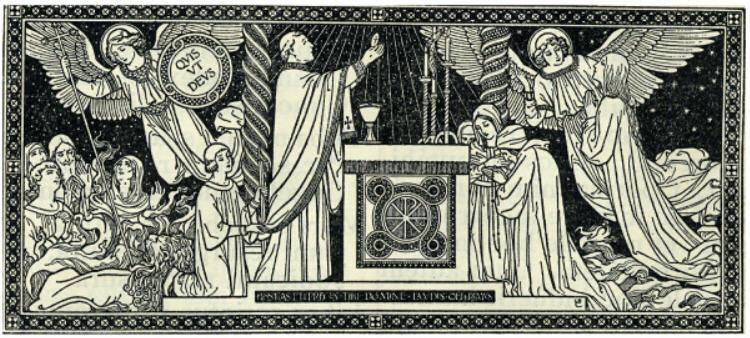
\includegraphics[width=\linewidth]{3.jpg}
				\end{figure}
						
				\section{MSZA ŚWIĘTA WIGILII PIĘCDZIESIĄTNICY}
			
					\rubric{
						Odnowiwszy w sobie łaskę Chrztu, który nas wszczepił w misterium śmierci i Zmartwychwstania Pańskiego, składamy ofiarę Mszy świętej, W tej Ofierze w sakramentalny sposób stanie się obecne misterium paschalne, to jest tajemnicze przejście Chrystusa przez śmierć do nowego życia. 
						Kapłan i usługujący ubrani w szaty mszalne koloru czerwonego udają się procesyjnie do ołtarza. W tym czasie chór kontynuuje Litanię, aż do końcowego Kyrie eleison. Teksty mszalne wysławiają działanie Ducha Świętego w duszy ochrzczonego i bierzmowanego. Działanie Ducha Św. Podobne jest do światła rozpraszającego ciemność i wody podtrzymującej życie na ziemi. Po okadzeniu ołtarza i odmówieniu Kyrie celebrans intonuje uroczyste Gloria, w podobny sposób jak w Wigilię Paschalną. Podczas hymnu dzwonią wszystkie dzwony.}
					
					\oremus{Kolekta}{
						Præsta, quæsumus, omnípotens Deus: ut claritatis tuæ super nos splendor effúlgeat; et lux tuæ lucis corda eórum, qui per grátiam tuam renáti sunt, Sancti Spíritus illustratióne confírmet.}{
						Wszechmogący Boże, spraw, niech zabłyśnie nad nami blask Twojej chwały, a światło Twej jasności niechaj umocni oświeceniem Ducha Świętego tych, którzy odrodzili się przez łaskę.}
					
					\proroctwoo{Epistoła (Dz 19:1--8)}
							{Uczniowie Jana Chrzciciela w Efezie przyjmują chrzest}
					
					\oremuss{
						In diébus illis: Factum est, cum Apóllo esset Corínthi, ut Paulus, peragrátis superióribus pártibus, veníret Ephesum et inveníret quosdam discípulos: dixítque ad eos: Si Spíritum Sanctum accepístis credéntes? At illi dixérunt ad eum: Sed neque, si Spíritus Sanctus est, audívimus. Ille vero ait: In quo ergo baptizáti estis? Qui dixérunt: In Ioannis baptísmate. Dixit autem Paulus: Ioánnes baptizávit baptísmo p\oe niténtiæ pópulum, dicens: In eum, qui ventúrus esset post ipsum, ut créderent, hoc est in Iesum. His audítis, baptizáti sunt in nómine Dómini Iesu. Et cum ímposuísset illis manus Paulus, venit Spíritus Sanctus super eos, et loquebántur linguis, et prophetábant. Erant autem omnes viri fere duódecim. Introgréssus autem synagógam, cum fidúcia loquebátur per tres menses, dísputans et suádens de regno Dei.}{
						W owym czasie, kiedy Apollos znajdował się w Koryncie, Paweł przeszedł okolice wyżej położone, przybył do Efezu i znalazł jakichś uczniów. Zapytał ich: «Czy otrzymaliście Ducha Świętego, gdy przyjęliście wiarę?» A oni do niego: «Nawet nie słyszeliśmy, że istnieje Duch Święty». «Jaki więc chrzest przyjęliście?» - zapytał.
						A oni odpowiedzieli: «Chrzest Janowy». «Jan udzielał chrztu nawrócenia, przemawiając do ludu, aby uwierzyli w Tego, który za nim idzie, to jest Jezusa» - powiedział Paweł. Gdy to usłyszeli, przyjęli chrzest w imię Pana Jezusa. A kiedy Paweł włożył na nich ręce, Duch Święty zstąpił na nich. Mówili też językami i prorokowali. Wszystkich ich było około dwunastu mężczyzn. Następnie wszedł do synagogi i odważnie przemawiał przez trzy miesiące rozprawiając i przekonując o królestwie Bożym.}
					
					\oremus{Alleluja (Ps 106:1, 116:1--2)}{
						\vv Confitémini Dómino, quóniam bonus: quóniam in s\ae culum misericordia eius.
						Laudáte Dóminum, omnes gentes: et collaudáte eum, omnes pópuli, \\
						\vv Quóniam confirmáta est super nos misericórdia eius: et véritas Dómini manet in ætérnum.}{
						\vv Sławcie Pana, bo jest dobry, bo na wieki miłosierdzie Jego.
						Chwalcie Pana, wszystkie narody, wysławiajcie Go, wszystkie ludy.\\
						\vv Bo Jego miłosierdzie nad nami utwierdzone, a wierność Pańska trwa na wieki.}
					
					\proroctwoo{Ewangelia (J 14:15--21)}{Duch Prawdy pozostanie z uczniami Jezusa}
					
					\oremuss{
						In illo témpore: Dixit Iesus discípulis suis: Si dilígitis me, mandáta mea serváte. Et ego rogábo Patrem, et alium Paráclitum dabit vobis, ut máneat vobíscum in ætérnum, Spíritum veritátis, quem mundus non potest accípere, quia non videt eum nec scit eum. Vos autem cognoscétis eum: quia apud vos manébit et in vobis erit. Non relínquam vos órphanos: véniam ad vos. Adhuc módicum: et mundus me iam non videt. Vos autem vidétis me, quia ego vivo, et vos vivétis, In illo die vos cognoscétis, quia ego sum in Patre meo, et vos in me, et ego in vobis. Qui habet mandáta mea et servat ea: ille est, qui díligit me. Qui autem díligit me, diligétur a Patre meo: et ego díligam eum, et manifestábo ei meípsum.}{
						W owym czasie rzekł Jezus swoim uczniom: «Jeż eli Mnie miłujecie, będziecie zachowywać moje przykazania. Ja zaś będę prosił Ojca, a innego Pocieszyciela da wam, aby z wami był na zawsze - Ducha Prawdy, którego ś wiat przyjąć nie moż e, ponieważ Go nie widzi ani nie zna. Ale wy Go znacie, ponieważ u was przebywa i w was będzie. Nie zostawię was sierotami: Przyjdę do was. Jeszcze chwila, a ś wiat nie będzie już Mnie oglądał. Ale wy Mnie widzicie, ponieważ Ja żyję i wy żyć będziecie. W owym dniu poznacie, ż e Ja jestem w Ojcu moim, a wy we Mnie i Ja w was. Kto ma przykazania moje i zachowuje je, ten Mnie miłuje. Kto zaś Mnie miłuje, ten będzie umiłowany przez Ojca mego, a również Ja będę go miłował i objawię mu siebie».}
					
					\oremus{Offertorium (Ps 103:30--31)}{
						Emítte Spíritum tuum, et creabúntur, et renovábis fáciem terræ: sit glória Dómini in s\ae cula, allelúia.}{
						Ześlij Ducha Twojego, a powstanie życie i odnowisz oblicze ziemi: niech chwała Pańska trwa na wieki, alleluja.}
					
					\oremus{Pieśń}{
						1. Pamiątkę dnia świątecznego\\
						Zesłania Ducha Świętego\\
						Dziś z Kościołem obchodzimy\\
						Dawcę darów pieśnią czcimy\\
						Alleluja, alleluja.\\
						
						2. Co Ezechiel zwiastował,\\
						O czym Joel prorokował\\
						To na oczy wszelkie ciało\\
						W dzień świąteczny oglądało. All.\\ 
						
						3. Gdy Apostołowie mili \\
						W tym dniu rzem się modlili,\\
						Nad nimi się płomieniste\\
						Jawią języki ogniste. All.}{
						4. Boskim ogniem zapaleni,\\
						Duchem Swiętym napełnieni,\\
						Śmiało Wśród tłumu wielkiego\\
						Głoszą Ukrzyżowanego. All.\\ \\
						
						5. Święty Piotr jednym kazaniem,\\
						Ducha Świętego działaniem,\\
						Tak porusza słuchające,\\
						Że nawraca trzy tysiące. All.\\
						
						6. Dziwują się Elamici,\\
						Z ziem dalekich prozelici\\
						I Partowie i Medowie,\\
						Że ich słyszą w swojej mowie. All.}
					
					\oremus{Sekreta}{
						Múnera, qu\ae sumus, Dómine, obláta sanctífica: et corda nostra Sancti Spíritus illustratióne emúnda.}{
						Prosimy Cię, Panie, uświęć złożone dary i oczyść nasze serca światłem Ducha Świętego.}
					
					\oremus{Prefacja o Duchu Świętym}{
						Vere dignum et iustum est, æquum et salutáre, nos tibi semper et ubíque grátias ágere: Dómine sancte, Pater omnípotens, ætérne Deus: per Christum, Dóminum nostrum. Qui, hodiernia die ascéndens super omnes c\oe los \textbf{sedénsque ad déxteram tuam, promíssum Spíritum Sanctum in fílios adoptiónis effúdit}. Quaprópter profúsis gáudiis totus in orbe terrárum mundus exsúltat. Sed et supérnæ Virtútes atque angélicæ Potestátes hymnum glóriæ tuæ cóncinunt, sine fine dicéntes:}{
						Zaprawdę godne to i sprawiedliwe, słuszne i zbawienne, abyśmy zawsze i wszędzie Tobie składali dziękczynienie, Panie, Ojcze święty, wszechmogący, wieczny Boże: przez Chrystusa, Pana naszego. On to wstąpiwszy ponad wszystkie niebiosa \textbf{i siedząc na prawicy Twojej zesłał w dniu dzisiejszym obiecanego Ducha Świętego na przybrane dzieci}. Dlatego cały okrąg ziemi tonie w nadmiarze radości. Lecz i Moce niebieskie, i anielskie Potęgi śpiewają hymn ku Twojej chwale, wołając bez końca:}
					
					\rubric{W Kanonie następujące modlitwy ulegają zmianie:}
					
					\oremuss{
						Communicántes, \textbf{et diem sacratíssimum Pentecóstes celebrántes}, quo Spíritus Sanctus Apóstolis innúmeris linguis appáruit: sed et memóriam venerántes...\\ \\  \\
						Hanc igitur oblationem servitutis nostræ, set et cunctæ familiæ tuæ, quam tibi offerimus pro his quoque, \textbf{quos regenerare dignatus es ex aqua, et Spiritu Sancto, tribuens eis remissionem omnium peccatorum}, quǽsumus Domine, ut placatus accipias: diesque nostros in tua pace disponas, atque ab æterna damnatione nos eripi, et in electorum tuorum iubeas grege numberari. Per Christum Dominum nostrum. Amen.}{
						Zjednoczeni w Świętych Obcowaniu, \textbf{obchodzimy prześwięty dzień Pięćdziesiątnicy}, w którym Duch Święty ukazał się Apostołom pod postacią niezliczonych języków, i ze czcią wspominamy...\\ \\
						Prosimy Cię przeto, Panie, abyś łaskawie przyjął tę ofiarę od nas sług Twoich, jak również od całego ludu Twego; składamy Ci ją za tych także, \textbf{których raczyłeś odrodzić z wody i Ducha Świętego, udzielając im odpuszczenia wszystkich grzechów}; racz dni nasze pokojem swym napełnić, od potępienia wiecznego nas uchronić i do grona wybranych swoich zaliczyć. Przez Chrystusa, Pana naszego. Amen.
					}
				
					\oremus{Communio (J 7:37--39)}{
						Ultimo festivitátis die dicébat Iesus: Qui in me credit, flúmina de ventre eius fluent aquæ vivæ: hoc autem dixit de Spíritu, quem acceptúri erant credéntes in eum, allelúia, allelúia.}{
						W ostatnim dniu święta mówił Jezus: Kto wierzy we mnie, rzeki wody żywej popłyną z jego wnętrza. A to mówił o Duchu, którego otrzymać mieli wierzący weń, alleluja.}
					
					\vfill
					
					\centerline{\pgfornament[width=3cm]{106}}
					
					\vfill
					
					\newpage
					
%					\centerline{\rule{3cm}{1.2pt}}

					\vspace*{-2em}
					
					\oremus{Pieśń}{
						1. Oto są baranki młode,\\
						oto ci, co zawołali alleluja!\\
						Dopiero przyszli do zdrojów,\\
						światłością się napełnili,  \\
						Alleluja, alleluja!\\
						
						2. Na Baranka Pańskich godach,\\
						W szat świątecznych czystej bieli,  \\
						Po krwawego morza wodach\\
						Nieśmy Panu pieśń weseli.\\
						
						3. W swej miłości wiekuistej\\
						On nas swoją Krwią częstuje,\\
						Nam też Ciało swe przeczyste\\
						Chrystus kapłan ofiaruje.\\ 
					
						4. Na drzwi świętą Krwią skropione\\
						Anioł mściciel z lękiem wziera,\\
						Pędzi morze rozdzielone,\\
						Wrogów w nurtach swych pożera.}{
						5. Już nam Paschą Tyś jest Chryste,\\ 
						Wielkanocną też ofiarą,\\
						Tyś Przaśniki nasze czyste \\
						Dla dusz prostych z szczerą wiarą.\\ \\
						
						6. O Ofiaro niebios święta,\\
						Ty moc piekła pokonywasz,\\
						Zrywasz ciężkie śmierci pęta,\\
						Wieniec życia nam zdobywasz. \\
						
						7. Chrystus piekło pogromiwszy\\
						Swój zwycięski znak roztacza,\\
						Niebo ludziom otworzywszy\\
						Króla mroków w więzy wtłacza.\\ 
						
						8. Byś nam wiecznie, Jezu drogi, \\
						Wielkanocną był radością,\\
						Strzeż od grzechu śmierci srogiej \\
						Odrodzonych Twą miłością.}
					
						\begin{center}		
							9. Chwała Ojcu i Synowi, \\
							który z martwych żywy wstaje\\
							I Świętemu też duchowi \\
							Niech na wieki nie ustaje. \\ 
						\end{center}
					
					\oremus{Pieśń}{
						1. U drzwi Twoich stoję, Panie, \textbf{x2}\\
						czekam na Twe zmiłowanie. \textbf{x2} \\
						
						2. Który pod postacią chleba, \\
						prawdziwy Bóg jesteś z nieba.\\
						
						3. W tej Hostyi jest Bóg żywy, \\
						choć zakryty, lecz prawdziwy.\\
						
						4. W tym Najświętszym Sakramencie, \\
						obecny w każdym momencie.\\
						
						5. Jak wielki cud Bóg uczynił, \\
						gdy chleb w Ciało swe przemienił.}{
						6. A nam pożywać zostawił, \\
						ażeby nas przez to zbawił.\\
						
						7. Święty, Mocny, Nieśmiertelny, \\
						w Majestacie Swym niezmierny.\\
						
						8. Aniołowie się lękają, \\
						choć na Jego twarz patrzają.\\
						
						9. Wszyscy niebiescy Duchowie, \\
						lękają się i królowie.\\
						
						10. Niebo, ziemia ani morze, \\
						pojąć, co jest Bóg, nie może.}
					
					\newpage
					
					\oremus{Modlitwa po Komunii}{
						Sancti Spíritus, Dómine, corda nostra mundet infúsio: et sui roris íntima aspersióne fecúndet.}{
						Panie, niech tchnienie Ducha Świętego oczyści nasze serca i użyźni je rosą Jego łaski.}
					
%					\centerline{\rule{3cm}{1.2pt}}
					
					\oremus{Regina C\ae li}{
						Regina C\ae li, l\ae tare, alleluia, \\
						Quia quem meruisti portare, alleluia, \\
						Resurrexit, sicut dixit, alleluia, \\
						Ora pro nobis Deum, alleluia.}{	
						Królowo nieba, wesel się, alleluja, \\
						Bo Ten, któregoś nosiła, alleluja, \\
						Zmartwychwstał jak powiedział, alleluja, \\
						Módl się za nami do Boga, alleluja.}
					
%					\centerline{\rule{3cm}{1.2pt}}
					
				\vfill
				
				\centerline{\pgfornament[width=4cm]{82}}
				
				\vfill
					
				\subsection{HYMN DO DUCHA ŚWIĘTEGO}
				
					\rubric{
						Za publiczne odśpiewanie tego hymnu można w Uroczystość Pięćdziesiątnicy uzyskać odpust zupełny.}
					
					\oremuss{
						Veni Creator Spiritus,\\
						Mentes tuorum visita,\\
						Imple superna gratia,\\
						Qu\ae  tu creasti pectora.\\
						
						Qui diceris Paraclitus,\\
						Altissimi donum Dei,\\
						Fons vivus, ignis, caritas,\\
						Et spiritalis unctio.\\
						
						Tu septiformis munere,\\
						Digitus patern\ae  dexter\ae ,\\
						Tu rite promissum Patris,\\
						Sermone ditans guttura.\\
						
						Accende lumen sensibus:\\
						Infunde amorem cordibus:\\
						Infirma nostri corporis\\
						Virtute firmans perpeti.\\
						
						Hostem repellas longius,\\
						Pacemque dones protinus:\\
						Ductore sic te pr\ae vio\\
						Vitemus omne noxium.\\
						
						Per te sciamus da Patrem,\\
						Noscamus atque Filium,\\
						Teque utriusque Spiritum\\
						Credamus omni tempore.\\
						
						Deo Patri sit gloria,\\
						Et Filio, qui a mortuis\\
						Surrexit, ac Paraclito,\\
						In s\ae culorum s\ae cula.\\
						Amen.
					
						\vv Emiite Spiritum tuum et creabuntur, alleluia\\
						\rr Et renovabis faciem terr\ae , alleluia.}{
						O Stworzycielu Duchu przyjdź,\\
						Nawiedź dusz wiernych Tobie krąg,\\
						Niebieską łaskę zesłać racz,\\
						Sercom, co dziełem są Twych rąk.\\
						
						Pocieszycielem jesteś zwan,\\
						I Najwyższego Boga dar,\\
						Tyś namaszczeniem naszych dusz,\\
						Zdrój żywy, miłość, ognia żar.\\
						
						Ty darzysz łaską siedmiokroć.\\
						Bo moc prawicy Ojca masz,\\
						Przez Ojca obiecany nam,\\
						Mową wzbogacasz język nasz.\\
						
						Światłem rozjaśnij naszą myśl,\\
						W serca nam miłość świętą wlej,\\
						I wątłą słabość naszych ciał,\\
						Pokrzep stałością mocy Swej.\\
						
						Nieprzyjaciela odpędź w dal,\\
						I Twym pokojem obdarz wraz,\\
						Niech w drodze za przewodem Twym,\\
						Miniemy zło co kusi nas.\\
						
						Daj nam przez Ciebie Ojca znać,\\
						Daj, by i Syn poznany był,\\
						I Ciebie jedno Tchnienie Dwóch,\\
						Niech wyznajemy z wszystkich sił.\\
						
						Niech Bogu Ojcu chwała brzmi,\\
						Synowi, który zmartwychwstał,\\
						I Temu co pociesza nas,\\
						Niech hołd wieczystych płynie chwał — Amen.
					
						\vv Ześlij Ducha Twego, a powstanie życie, alleluja.\\
						\rr I odnowisz oblicze ziemi, alleluja.}
					
					\oremus{Modlitwa}{
						Deus, qui (hodiérna die) corda fidélium Sancti Spíritus illustratióne docuísti: da nobis in eódem
						Spíritu recta sápere; et de eius semper consolatióne gaudére...}{
						Boże, Ty (w dniu dzisiejszym) pouczyłeś serca wiernych światłem Ducha Świętego, daj nam w tymże Duchu poznać, co jest prawe i zawsze radować się Jego pociechą...}
					
					\oremus{Pieśń}{}{}
					
			 		Przez Twoje święte Ducha Zesłanie, Boży Synu! odpuść nam nasze zgrzeszenie: \\
					Wierzymy żeś Ducha zesłał, Żywoteś nas naprawił; \\
					Śmierci wiecznej nas zbawił, Śwoję świętą moc zjawił.
					
				\vfill
				
				\centerline{\pgfornament[width=7cm]{82}}
				
				\vfill
				
				\newpage
				
				\fancyhead[CE,CO]{NIEDZIELA PIĘĆDZIESIĄTNICY}
				
				\begin{figure}[h]
					\centering
					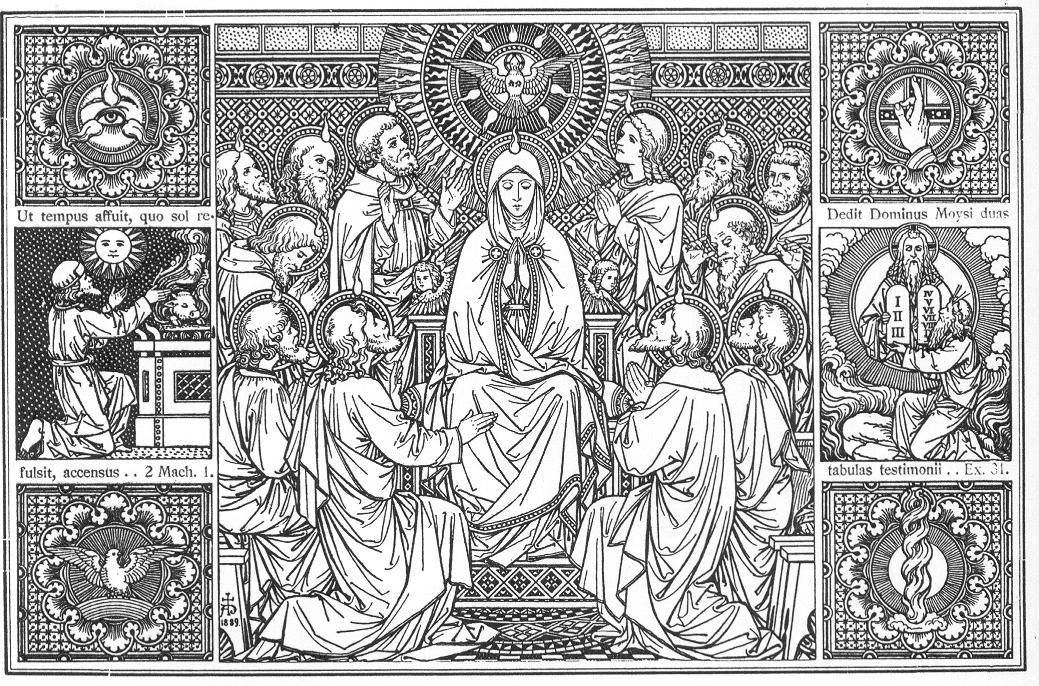
\includegraphics[width=\linewidth]{2.jpg}
				\end{figure}
			
				\section{NIEDZIELA PIĘĆDZIESIĄTNICY}
					{\station{Stacja u św. Piotra}}
					
				\rubric{
					W dzień Pięćdziesiątnicy około godziny dziewiątej przed południem Duch Święty zstąpił pod postacią wichru i ognia na uczniów zgromadzonych w wieczerniku. Msza świąteczna odprawiana w porze przedpołudniowej jest uroczystym obchodem rocznicy tego wydarzenia. Świadomi swojej słabości prosimy Ducha Świętego aby umocnił to, czego dokonały w nas sakramenty Chrztu i Bierzmowania i nieustannie obdarzał nas swoimi natchnieniami.}
				
				\oremus{Introit (Mdr 1:7, Ps 67:2)}{
					Spíritus Dómini replévit orbem terrárum, allelúia: et hoc quod cóntinet ómnia, sciéntiam habet vocis, allelúia, allelúia, allelúia.\\
					\vv Exsúrgat Deus, et dissipéntur inimíci eius: et fúgiant, qui odérunt eum, a fácie eius.\\}{
					Duch Pański napełnił okrąg ziemi, alleluja: A Ten, który wszystko obejmuje, zna każde słowo, alleluja, alleluja, alleluja.\\ \\
					\vv Bóg wstaje, a rozpraszają się Jego wrogowie i pierzchają przed Jego obliczem ci, którzy Go nienawidzą.}
				
				\newpage
				
				\oremus{Kolekta}{
					Deus, qui hodiérna die corda fidélium Sancti Spíritus illustratióne docuísti: da nobis in eódem Spíritu recta sápere; et de eius semper consolatióne gaudére.}{
					Boże, któryś w dniu dzisiejszym pouczył serca wiernych światłem Ducha Świętego, daj nam w tymże Duchu poznać co jest prawe i pociechą Jego zawsze się radować.}
				
				\proroctwoo{{Epistoła (Dz 2,1--11)}}{Wszyscy zostali napełnieni Duchem Świętym}
				
				\rubric{
					Dar języków jest potwierdzeniem powszechnej misji Kościoła. Wszystkie narody są wezwane do słuchania Dobrej Nowiny.}
				
				\oremuss{
					Cum compleréntur dies Pentecóstes, erant omnes discípuli pariter in eódem loco: et factus est repéente de c\oe lo sonus, tamquam adveniéntis spíritus veheméntis: et replévit totam domum, ubi erant sedentes. Et apparuérunt illis dispertítæ linguæ tamquam ignis, sedítque supra síngulos eórum: et repléti sunt omnes Spíritu Sancto, et c\oe pérunt loqui váriis linguis, prout Spíritus Sanctus dabat éloqui illis. Erant autem in Ierúsalem habitántes Iud\ae i, viri religiósi ex omni natióne, quæ sub c\oe lo est. Facta autem hac voce, convénit multitúdo, et mente confúsa est, quóniam audiébat unusquísque lingua sua illos loquéntes. Stupébant autem omnes et mirabántur, dicéntes: Nonne ecce omnes isti, qui loquúntur, Galil\ae i sunt? Et quómodo nos audívimus unusquísque linguam nostram, in qua nati sumus? Parthi et Medi et Ælamítæ et qui hábitant Mesopotámiam, Iud\ae am et Cappadóciam, Pontum et Asiam, Phrýgiam et Pamphýliam, Ægýptum et partes Líbyæ, quæ est circa Cyrénen, et ádvenæ Románi, Iud\ae i quoque et Prosélyti, Cretes et Arabes: audívimus eos loquéntes nostris linguis magnália Dei.}{
					Kiedy nadszedł dzień Pięćdziesiątnicy, znajdowali się wszyscy razem na tym samym miejscu. Nagle spadł z nieba szum, jakby uderzenie gwałtownego wiatru, i napełnił cały dom, w którym przebywali. Ukazały się im też języki jakby z ognia, które się rozdzieliły, i na każdym z nich spoczął jeden. I wszyscy zostali napełnieni Duchem Świętym, i zaczęli mówić obcymi językami, tak jak im Duch pozwalał mówić. 
					Przebywali wtedy w Jerozolimie pobożni Żydzi ze wszystkich narodów pod słońcem. Kiedy więc powstał ów szum, zbiegli się tłumnie i zdumieli, bo każdy słyszał, jak przemawiali w jego własnym języku. 
					Pełni zdumienia i podziwu mówili: ”Czyż ci wszyscy, którzy przemawiają, nie są Galilejczykami? Jakżeż więc każdy z nas słyszy swój własny język ojczysty? – Partowie i Medowie, i Elamici, i mieszkańcy Mezopotamii, Judei oraz Kapadocji, Pontu i Azji, Frygii oraz Pamfilii, Egiptu i tych części Libii, które leżą blisko Cyreny, i przybysze z Rzymu, Żydzi oraz prozelici, Kreteńczycy i Arabowie – słyszymy ich głoszących w naszych językach wielkie dzieła Boże”. }
				
				\newpage
				
				\proroctwo{Alleluja(Ps 103:30)}
				
				\rubric{Na słowa \textit{Veni Sancte Spiritus} przyklęka sie.}
				
				\oremuss{
					Allelúia, allelúia\\
					Emítte Spíritum tuum, et creabúntur, et renovábis fáciem terræ. Allelúia\\
					\vv Veni, Sancte Spíritus, reple tuórum corda fidélium: et tui amóris in eis ignem accénde.}{
					Alleluja, alleluja\\
					Ześlij Ducha Twojego, a powstanie życie i odnowisz oblicze ziemi, alleluja. \\
					\vv Przyjdź, Duchu Święty, napełnij serca Twych wiernych i zapal w nich ogień Twojej miłości.}
				
				\proroctwo{Sekwencja}
				
				\rubric{
					Błagalna sekwencja w poetyckiej formie opisuje działanie Ducha Świętego w duszach wiernych.}
				
				\oremuss{
					Veni, Sancte Spíritus, \\
					et emítte c\ae litus \\
					lucis tuæ rádium.\\
					
					Veni, pater páuperum; \\
					veni, dator múnerum; \\
					veni, lumen córdium.\\
					
					Consolátor óptime, \\
					dulcis hospes ánimæ, \\
					dulce refrigérium.\\
					
					In labóre réquies, \\
					in æstu tempéries, \\
					in fletu solácium.\\
					
					O lux beatíssima, \\
					reple cordis íntima \\
					tuórum fidélium.\\
					
					Sine tuo númine \\
					nihil est in hómine, \\
					nihil est innóxium.\\
					
					Lava quod est sórdidum, \\
					riga quod est áridum, \\
					sana quod est sáucium.
					
					Flecte quod est rígidum, \\
					fove quod est frígidum, \\
					rege quod est dévium.\\
					
					Da tuis fidélibus, \\
					in te confidéntibus, \\
					sacrum septenárium.\\
					
					Da virtútis méritum, \\
					da salútis éxitum, \\
					da perénne gáudium. \\
					Amen. Allelúia.}{
					Przybądź, Duchu Święty,\\
					Spuść z niebiosów wzięty \\
					Światła Twego strumień. \\
					
					Przyjdź, Ojcze ubogich,\\
					Przyjdź, Dawco łask drogich, \\
					Przyjdź, światłości sumień. \\
					
					O najmilszy z gości, \\
					Słodka serc radości, \\
					Słodkie orzeźwienie!\\
					
					W pracy Tyś ochłodą, \\
					W skwarze żywą wodą, \\
					W płaczu utulenie.\\
					
					Światłości najświętsza, \\
					Serc wierzących wnętrza \\
					Poddaj Twej potędze. \\
					
					Bez Twojego tchnienia \\
					Cóż jest wśród stworzenia, \\
					Jeno cierń i nędze. \\
					
					Obmyj, co nieświęte, \\
					Oschłym wlej zachętę, \\
					Ulecz serca ranę. 
					
					Nagnij, co jest harde, \\
					Rozgrzej serca twarde, \\
					Prowadź zabłąkane. \\
					
					Daj Twoim wierzącym,\\
					W Tobie ufającym \\
					Siedmiorakie dary. \\
					
					Daj zasługę męstwa,\\
					Daj wieniec zwycięstwa,\\
					Daj szczęście bez miary.\\
					Amen. Alleluja.}
				
				\proroctwoo{Ewangelia (J 14, 23--31)}{Zapowiedź Ducha Pocieszyciela}
				
				\oremuss{
					In illo témpore: Dixit Iesus discípulis suis: Si quis díligit me, sermónem meum servábit, et Pater meus díliget eum, et ad eum veniémus et mansiónem apud eum faciémus: qui non díligit me, sermónes meos non servat. Et sermónem quem audístis, non est meus: sed eius, qui misit me, Patris. Hæc locútus sum vobis, apud vos manens. Paráclitus autem Spíritus Sanctus, quem mittet Pater in nómine meo, ille vos docébit ómnia et súggeret vobis ómnia, quæcúmque díxero vobis. Pacem relínquo vobis, pacem meam do vobis: non quómodo mundus dat, ego do vobis. Non turbátur cor vestrum neque formídet. Audístis, quia ego dixi vobis: Vado et vénio ad vos. Si diligere tis me, gaudere tis utique, quia vado ad Patrem: quia Pater maior me est. Et nunc dixi vobis, priúsquam fiat: ut, cum factum fúerit, credátis. Iam non multa loquar vobíscum. Venit enim princeps mundi huius, et in me non habet quidquam. Sed ut cognóscat mundus, quia díligo Patrem, et sicut mandátum dedit mihi Pater, sic fácio.}{\vspace*{-3pt}
					W owym czasie rzekł Jezus swoim uczniom: Kto ma przykazania moje i zachowuje je, ten Mnie miłuje. Kto zaś Mnie miłuje, ten będzie umiłowany przez Ojca mego, a również Ja będę go miłował i objawię mu siebie».  Rzekł do Niego Juda, ale nie Iskariota: «Panie, cóż się stało, że nam się masz objawić, a nie światu?» W odpowiedzi rzekł do niego Jezus: «Jeśli Mnie kto miłuje, będzie zachowywał moją naukę, a Ojciec mój umiłuje go, i przyjdziemy do niego, i będziemy u niego przebywać. Kto Mnie nie miłuje, ten nie zachowuje słów moich. A nauka, którą słyszycie, nie jest moja, ale Tego, który Mnie posłał, Ojca. To wam powiedziałem przebywając wśród was. A Pocieszyciel, Duch Święty, którego Ojciec pośle w moim imieniu, On was wszystkiego nauczy i przypomni wam wszystko, co Ja wam powiedziałem.  Pokój zostawiam wam, pokój mój daję wam. Nie tak jak daje świat, Ja wam daję. Niech się nie trwoży serce wasze ani się lęka!  Słyszeliście, że wam powiedziałem: Odchodzę i przyjdę znów do was. Gdybyście Mnie miłowali, rozradowalibyście się, że idę do Ojca, bo Ojciec większy jest ode Mnie. A teraz powiedziałem wam o tym, zanim to nastąpi, abyście uwierzyli, gdy się to stanie. Już nie będę z wami wiele mówił, nadchodzi bowiem władca tego świata Nie ma on jednak nic swego we Mnie. Ale niech świat się dowie, że Ja miłuję Ojca, i że tak czynię, jak Mi Ojciec nakazał.}
				
				\oremus{Offertorium (Ps 67:29--30)}{
					Confírma hoc, Deus, quod operátus es in nobis: a templo tuo, quod est in Ierúsalem, tibi ófferent reges múnera, allelúia}{
					Utwierdź to, Boże, czegoś w nas dokonał. Przez wzgląd na Twoją świątynię, która jest w Jeruzalem, niech królowie złożą Ci dary, alleluja.}
				
				\oremus{Sekreta}{
					Múnera, qu\ae sumus, Dómine, obláta sanctífica: et corda nostra Sancti Spíritus illustratióne emúnda.}{
					Prosimy Cię, Panie, uświęć złożone dary i oczyść nasze serca światłem Ducha Świętego.}
				
				\rubric{
					Prefacja o Duchu Świętym. W Kanonie odmawia się własne modlitwy, tak jak podczas Wigilii.}
				
				\oremus{Communio (Dz 2:2; 2:4)}{
					Factus est repénte de c\oe lo sonus, tamquam adveniéntis spíritus veheméntis, ubi erant sedéntes, allelúia: et repléti sunt omnes Spíritu Sancto, loquéntes magnália Dei, allelúia, allelúia.}{
					Nagle dał się słyszeć z nieba szum jakby nadchodzącego wichru gwałtownego tam gdzie przebywali, alleluja. I wszyscy zostali napełnieni Duchem Świętym i mówili o wielkich sprawach Bożych, alleluja, alleluja.}
				
				\oremus{Modlitwa po Komunii}{
					Sancti Spíritus, Dómine, corda nostra mundet infúsio: et sui roris íntima aspersióne fecúndet.}{
					Panie, niech tchnienie Ducha Świętego oczyści nasze serca, i użyźni je rosą Jego łaski.}
				
				\vfill
				
				\centerline{\pgfornament[width=7cm]{82}}
				
				\vfill
				
			
\end{document}







